% !BIB TS-program = biber

\RequirePackage[l2tabu,orthodox]{nag}

% TODO: decide if one-sided/two-sided
%\documentclass[headsepline,footsepline,footinclude=false,fontsize=11pt,paper=a4,listof=totoc,bibliography=totoc,BCOR=12mm,DIV=12]{scrbook} % two-sided
\documentclass[headsepline,footsepline,footinclude=false,oneside,fontsize=11pt,paper=a4,listof=totoc,bibliography=totoc]{scrbook}
\usepackage{amsmath}
\usepackage{amsopn}
\usepackage{amstext}
\usepackage{multirow} % one-sided

% TODO: change thesis information
\newcommand*{\getUniversity}{Technische Universität München}
\newcommand*{\getFaculty}{Informatics}
\newcommand*{\getDegree}{Informatics}
\newcommand*{\getSchool}{Computation, Information and Technology}
\newcommand*{\getTitle}{Investigation of Convolutional Neural Networks for Iterative Solver Selection}
\newcommand*{\getTitleGer}{Untersuchung von Convolutional Neural Networks zur Auswahl iterativer Löser}
\newcommand*{\getAuthor}{Leon Unterberger}
\newcommand*{\getDoctype}{Bachelor's Thesis}
\newcommand*{\getSupervisor}{Bungartz, Hans-Joachim}
\newcommand*{\getAdvisor}{Liu Weng, Hayden}
\newcommand*{\getKeywords}{CNN, iterative solvers, solver selection}
\newcommand*{\getSubmissionDate}{23.07.2026}
\newcommand*{\getSubmissionLocation}{Munich}

% TODO: change citation style in settings
\input{settings}

\begin{document}

% Set page numbering to avoid "destination with the same identifier has been already used" warning for cover page.
% (see https://en.wikibooks.org/wiki/LaTeX/Hyperlinks#Problems_with_Links_and_Pages).
\pagenumbering{alph}
\input{pages/cover}

\frontmatter{}

\input{pages/title}
\input{pages/disclaimer}
\thispagestyle{empty}
\chapter*{Declaration of AI Usage}

The following AI tools were used during the preparation of this thesis:

\begin{itemize}
  \item \textbf{Claude Code (Claude Sonnet 4.6, Anthropic, accessed 2025--2026)} was used
        throughout the development of the experimental pipeline.
        This includes assistance with writing, debugging, and refactoring Python scripts for
        data generation, model training, and evaluation, as well as help with
        Docker configuration and \LaTeX{} formatting.
        All generated code was reviewed, tested, and in many parts written or substantially
        modified by me.

  \item \textbf{Claude (Claude Sonnet 4.6, Anthropic, accessed 2025--2026)} was used
        for structural guidance during thesis writing, such as organising sections and
        suggesting what content belongs in each chapter.
        It was also used for proofreading drafts and identifying unclear passages.
        All text in the final thesis was written or rewritten by me;
        no AI-generated text was included verbatim.
\end{itemize}

AI tools were not used to generate experimental results, to interpret data on my behalf, or to
produce any figures. The scientific content, the analysis of results, and all conclusions are
entirely my own work.

\vspace{15mm}
\noindent
\getSubmissionLocation{}, \getSubmissionDate{} \hspace{\fill} \getAuthor{}

\cleardoublepage{}

% Uncomment the following line if you want to include a software usage table (see example in pages/software_used.tex)
% \input{pages/software_used}
% \input{pages/acknowledgments}
\chapter{\abstractname}

Selecting the right solver and preconditioner for large sparse linear systems $Ax=b$ is critical for computational efficiency across many scientific and engineering fields.
This process requires significant domain expertise or costly benchmarking.
MM-AutoSolver demonstrated that a multimodal CNN+MLP architecture combining a sparsity-pattern image with matrix features can automate this selection.

This thesis extends that approach by systematically evaluating 14 image encoding strategies at different resolutions, introducing dual-channel CNN inputs that use pairs of image encodings in parallel, a convergence penalty to reduce solver failure rates, and an ensemble of independently trained models.

The key finding is that magnitude-based image encodings consistently outperform other encoding methods.
Combining it with a complementary image mode in the dual-channel CNN input increases F1 by 2.2\% over the best single-channel approach.
An ensemble of four dual-channel models achieves a 66.77\% macro F1, surpassing the MM-AutoSolver approach by approximately 4\% in F1 despite a harder, more balanced dataset.


% % !TeX root = ../main.tex

\chapter{Zusammenfassung}

%TODO: Zusammenfassung (German summary)
 German summary is not needed
\microtypesetup{protrusion=false}
\tableofcontents{}
\microtypesetup{protrusion=true}

\mainmatter{}

%\addchap{Abbreviations}

% !TeX root = ../main.tex
% Add the above to each chapter to make compiling the PDF easier in some editors.

\chapter{Introduction}\label{chapter:introduction}

\section{Motivation}\label{sec:motivation}

Linear systems of equations in the form $Ax=b$ arise across nearly every domain in computer science, from structural mechanics and fluid dynamics to machine learning and network analysis.
While small systems can be solved directly with Gaussian elimination in \(\mathcal{O}(n^3)\) time, real-world problems often generate sparse matrices with thousands or millions of unknowns where direct methods become unfeasible.
Such matrices are called sparse because the vast majority of their $n^2$ entries are zero, only a small fraction $\text{nnz} \ll n^2$ are non-zero.
Iterative solvers, such as Conjugate Gradient (CG), Generalized Minimal Residual (GMRES), or Flexible Generalized Minimal Residual (FGMRES), are practical alternatives.
They exploit sparsity and can converge in far fewer operations than direct methods, but their performance for a given problem depends on the chosen combination of solver and preconditioner.

Selecting the best solver-preconditioner pair for a concrete problem is not easy.
A configuration that converges in hundreds of iterations for a symmetric positive definite system from a finite-element discretisation may stagnate entirely on an indefinite or non-symmetric problem.
Practitioners today rely on mathematical knowledge, trial and error, or specific benchmarking, which require significant manual effort in every step.
Automating or improving this selection step is therefore an important open problem, which this thesis addresses.

\section{Research Gap and Problem Statement}\label{sec:research-gap}

Recent work has shown that machine learning models can predict good solver--preconditioner pairs from matrix properties alone.
In particular, Xiong et al.\ \cite{xiong2025mmautosolver} proposed \emph{MM-AutoSolver}, a multimodal CNN+MLP framework that encodes both a sparsity-pattern image and a hand-crafted feature vector to classify the best solver.
They report 78.54\% accuracy on a benchmark dataset of 11{,}623 matrices, including real-world application matrices from SuiteSparse~\cite{davis2011university}, FreeFEM~\cite{hecht2012freefem}, and OpenFOAM~\cite{weller1998tensorial}.
Weng et al.~\cite{weng2026embedding} take a complementary approach, learning solver--problem relationships directly from observed performance data rather than engineering features by hand.
A detailed survey of both works is given in \autoref{chapter:related-work}.

Several gaps remain in the MM-AutoSolver approach, however:

\begin{itemize}
  \item \textbf{Limited feature study.} MM-AutoSolver uses 17 fixed features; the sensitivity to feature choice and the benefit of additional structural descriptors (e.g.\ diagonal dominance variance, structural symmetry) has not been studied.
  \item \textbf{Single image mode.} Only a density representation at 128\,px is evaluated, it is unknown whether other encodings (magnitude, sign, RCM-reordered variants) carry complementary information.
  \item \textbf{No multi-channel fusion.} Combining two image modes as a dual-channel input has not been explored.
  \item \textbf{Convergence failures unpenalised.} Standard cross-entropy loss does not discourage predictions that select non-converging solvers, which may lead to costly timeouts in practice.
  \item \textbf{No ensemble evaluation.} The benefit of averaging predictions from multiple independently trained models has not been quantified.
\end{itemize}

\section{Research Goals and Contributions}\label{sec:contributions}

This thesis pursues the following goals:

\begin{enumerate}
  \item \textbf{Replication.} Re-implement MM-AutoSolver as a controlled baseline to verify and contextualize the reported results on an independently generated dataset.
  \item \textbf{Feature engineering.} Choose a different set of 14 base matrix descriptors than MM-AutoSolver and extend it to 20, measuring the impact on classification accuracy.
  \item \textbf{Image mode study.} Train and compare 14 single-channel image representations (binary, density, magnitude, sign, symmetry, diagonal, signed\_magnitude, and their RCM-reordered counterparts) at 64\,px and 128\,px.
  \item \textbf{Dual-channel CNN.} Fuse pairs of the best-performing modes into a two-channel input and evaluate pairwise combinations at different resolutions.
  \item \textbf{Convergence penalty.} Introduce a loss term that penalizes probability mass assigned to non-converging solvers and evaluate its effect on failure rate.
  \item \textbf{Ensemble evaluation.} Average softmax outputs from multiple top models and measure the accuracy gain over any individual model.
\end{enumerate}

\section{Thesis Structure}\label{sec:structure}

The remainder of this thesis is organised as follows.
\autoref{chapter:related-work} surveys existing work on iterative solver selection and the MM-AutoSolver baseline.
\autoref{chapter:methodology} describes the dataset, model architecture, training procedure, and evaluation protocol.
\autoref{chapter:experiments} details each experimental campaign in turn.
\autoref{chapter:results} analyses and compares the results across all configurations.
\autoref{chapter:conclusion} summarises the findings, discusses limitations, and outlines directions for future work.

% !TeX root = ../main.tex
% Add the above to each chapter to make compiling the PDF easier in some editors.

\chapter{Related Work}\label{chapter:related-work}

\section{Iterative Solvers and Preconditioners}\label{sec:solvers-background}

Iterative methods for sparse linear systems construct a sequence of approximations to the
solution of $Ax = b$ by building a Krylov subspace
$\mathcal{K}_k(A, r_0) = \operatorname{span}\{r_0,\, Ar_0,\, \ldots,\, A^{k-1}r_0\}$
from the initial residual $r_0$.
The Conjugate Gradient method (CG) is the standard choice for symmetric positive definite
systems, while methods such as GMRES, FGMRES, DGMRES, BiCGStab, and BiCGStabl handle
non-symmetric or indefinite problems.
Further specialisations include MINRES for symmetric indefinite systems, as well as CR and
CGS for specific structural properties.
A comprehensive treatment of Krylov subspace methods is given by Saad~\cite{saad2003iterative}.

Preconditioners transform the linear system to improve convergence by approximating
$A^{-1}$ at low computational cost.
Simple diagonal methods such as Jacobi, SOR, and the Eisenstat variant are inexpensive but
effective for diagonally dominant systems.
Incomplete LU factorisation (ILU), introduced by Meijerink and Van der
Vorst~\cite{meijerink1977iterative}, approximates the LU decomposition while discarding
small fill-in entries, offering a stronger approximation at moderate cost.
Block variants such as block Jacobi and additive Schwarz (ASM) decompose the system into
local subproblems that can be solved independently or in parallel.
Algebraic multigrid (AMG and its PETSc implementation GAMG) constructs a hierarchy of
coarser representations and achieves near-optimal convergence for a wide class of
problems~\cite{stuben2001review}.
Because no single solver-preconditioner pair dominates across all matrix types, selecting
the right combination requires problem-specific knowledge, which motivates automated
selection.

\section{Automated Solver Selection}\label{sec:automated-selection}

Automating the choice of solver and preconditioner has been studied from several angles.
Rule-based expert systems encode practitioner knowledge about which configurations suit
which matrix properties, but are limited to known problem classes and require significant
manual effort to maintain.
Classical machine learning approaches overcome this by training classifiers such as support
vector machines or random forests on hand-crafted matrix statistics, learning the mapping
from matrix properties to optimal solver configurations directly from benchmark data.

More recent work extends this idea to richer input representations.
MM-AutoSolver~\cite{xiong2025mmautosolver} supplements scalar matrix features with a CNN
branch processing a visual rendering of the sparsity pattern, improving accuracy over
feature-only baselines.
Weng et al.~\cite{weng2026embedding} take a different direction with an embedding-based
framework that learns solver-problem relationships directly from observed performance data,
achieving substantial improvements over classical feature-based models across a broad set
of PETSc solver-preconditioner configurations.

\section{MM-AutoSolver}\label{sec:mm-autosolver}

MM-AutoSolver~\cite{xiong2025mmautosolver} is the primary baseline and architectural
reference for this thesis.
The model combines two input streams: a scalar feature branch processing 17 hand-crafted
matrix statistics through an MLP, and a CNN branch operating on a $128 \times 128$ pixel
density image of the sparse matrix.
The two branches are fused via element-wise addition before a shared classification head
predicts one of 19 fixed solver-preconditioner pairs from PETSc~\cite{dalcin2011parallel}.
The CNN uses two convolutional layers with Tanh activations and $3 \times 3$ and
$5 \times 5$ kernels respectively, trained with Adam ($\text{lr} = 10^{-3}$,
256 epochs, batch size 512).
On a dataset of 11{,}623 matrices from the SuiteSparse collection~\cite{davis2011university} the model achieves Acc\,=\,78.54\,\%,
MP\,=\,63.41\,\%, MR\,=\,62.81\,\%, and F1\,=\,62.53\,\%.
This thesis independently replicates MM-AutoSolver on a custom dataset~(\autoref{sec:mm-replication})
and extends the approach by systematically evaluating 14 different image encoding strategies,
dual-channel CNN inputs, and ensemble methods.

\section{Embedding-based Solver Performance Prediction}\label{sec:supervisor-framework}

Weng et al.~\cite{weng2026embedding} present an embedding-based framework for linear solver
performance prediction evaluated across 101 PETSc solver-preconditioner configurations on
a broad set of SuiteSparse benchmark matrices.
Rather than engineering features by hand, the framework learns solver-problem relationships
directly from observed performance data and projects unseen problems into a learned
embedding space using inexpensive numerical features, achieving a 37\,\% reduction in mean
average percentage error and a 17\,\% improvement in top-prediction accuracy over classical
feature-based models.
This thesis targets a subset of 19 of the 101 solver-preconditioner configurations from
this framework as classification labels, with the goal of training a CNN-based model that
could eventually serve as a lightweight inference module within the broader
evaluation pipeline.

\section{Image Representations of Sparse Matrices}\label{sec:image-representations}

Representing a sparse matrix as a two-dimensional image allows a CNN to exploit spatial
and structural patterns that scalar statistics cannot capture.
The simplest encoding is a binary sparsity pattern, marking each non-zero entry as a pixel.
Denser representations encode the value magnitude or local non-zero density per pixel cell,
optionally on a logarithmic scale to compress dynamic range; signed variants additionally
preserve entry signs.
Before rendering, the Reverse Cuthill--McKee (RCM) reordering~\cite{cuthill1969reducing}
reduces the matrix bandwidth by permuting rows and columns, concentrating non-zero entries
closer to the diagonal and making structural patterns more visually compact.
MM-AutoSolver~\cite{xiong2025mmautosolver} uses a single density encoding at
$128 \times 128$ pixels; this thesis evaluates 14 distinct encoding strategies at two
resolutions to identify the most informative representation for solver selection.

\section{Convolutional Neural Networks and Multimodal Learning}\label{sec:cnn-background}

Convolutional neural networks learn hierarchical spatial features from image data and are
well established for image classification tasks.
In this thesis, the CNN serves as one branch of a multimodal architecture that combines
image and scalar inputs.
Multimodal machine learning, as surveyed by Baltru\v{s}aitis et
al.~\cite{baltruvsaitis2018multimodal}, combines complementary signals from multiple input
modalities to improve prediction over any single modality alone.
The dual-stream design used here follows this paradigm: the CNN branch captures spatial
matrix structure while the MLP branch processes scalar statistics, and the two sources of
information are fused through concatenation before a shared classification head.

% !TeX root = ../main.tex
% Add the above to each chapter to make compiling the PDF easier in some editors.

\chapter{Methodology}\label{chapter:methodology}

This chapter covers which problem the thesis tackles, how the data used within the different experiments is generated, what the actual data looks like,
which solver-preconditioner classes are used, which features are selected and why, and describes the architecture used in the PyTorch model.

\section{Problem Formulation}\label{sec:problem-formulation}

The goal of the thesis is to evaluate the usability of CNNs for a pipeline that tries to predict the solver-preconditioner
pair that minimises solve time subject to convergence in a large sparse equation in the form of $Ax = b$, where
$A \in \mathbb{R}^{n \times n}$, $b \in \mathbb{R}^{n \times 1}$, and $x \in \mathbb{R}^{n \times 1}$.
To determine the usability an architecture similar to that in the MM-AutoSolver~\cite{xiong2025mmautosolver} paper is introduced initially, which is
then modified in certain aspects like the chosen features and the approach of the CNN implementation.
These changes are done with the goal in mind to achieve the best possible prediction outcome while also improving the overall failure rates and average speedups
of the resulting models which allows them to be used in a complete pipeline.

\section{Dataset Construction}\label{sec:dataset}

The dataset is constructed by combining SuiteSparse~\cite{davis2011university} matrices with synthetically generated matrices and saving the information needed for
further processing into an HDF5 file.
For the dataset a cap on winning solver-preconditioner pairs is introduced to counter a certain bias towards overrepresented pairs in the training phase.
For the dataset used in the experiments this cap was 600, while the minimum of wins for a pair was 250.

\subsection{Synthetic Data Generation}\label{subsec:synthetic-datagen}

The synthetic data generation evolved while testing and generating datasets, in the end 37 different generator buckets
were defined in the process.
These focus on generating matrices with structural properties for which specific solver-preconditioner pairs are theoretically expected to perform well;
the actual winner is always determined empirically by benchmarking.
Table~\ref{tab:generator-buckets} lists all generator functions grouped by structural property.
In practice, however, this worked only partially, as even though some solver wins increased, in most cases the intended target solvers were still
outperformed by certain more dominant solver-preconditioner pairs.
A more systematic bucket design falls outside the scope of this thesis and these downsides are therefore accepted as limitations.
For generators where only the size changes which solver-preconditioner pair has the highest chance of winning, different buckets
that generate specific sizes with a certain generator function are introduced.
If these generators produce large matrices, they have a lower chance to be used as they
dramatically increase the runtime of the data generation.
In the current state, the generators generate matrices with $n$ ranging from 100 to 125{,}000.

\begin{table}[H]
  \centering
  \caption{Synthetic generator buckets grouped by structural matrix property.
           Size variants of the same generator function are merged into one row.
           Solver requirements follow~\cite{saad2003iterative}: CG requires SPD (Ch.\,6),
           MINRES/SYMMLQ require symmetry (Ch.\,6), GMRES and BiCGS variants apply to
           nonsymmetric systems (Ch.\,7).
           Primary targets are theoretically motivated and empirically confirmed.}
  \label{tab:generator-buckets}
  \small
  \begin{tabular}{@{}llp{4.5cm}@{}}
    \toprule
    \textbf{Generator function} & \textbf{$n$ range} & \textbf{Primary target(s)} \\
    \midrule
    \multicolumn{3}{@{}l@{}}{\textit{Symmetric positive-definite (SPD)}} \\[2pt]
    \texttt{random\_spd}               & 100–1\,000      & \texttt{cg+\{ilu, eisenstat, bjacobi\}} \\
    \texttt{poisson\_2d}               & 100–90\,000     & \texttt{cg+*, minres+gamg, fcg+gamg} \\
    \texttt{poisson\_3d}               & 125–125\,000    & \texttt{cg+*, minres+gamg, fcg+gamg} \\
    \texttt{anisotropic\_poisson\_2d}  & 100–40\,000     & \texttt{cg+ilu, fcg+gamg} \\
    \texttt{anisotropic\_poisson\_3d}  & 1\,700–27\,000  & \texttt{fcg+gamg} \\
    \midrule
    \multicolumn{3}{@{}l@{}}{\textit{Symmetric indefinite}} \\[2pt]
    \texttt{shifted\_spd}              & 100–10\,000     & \texttt{symmlq+*, cr+*} \\
    \texttt{helmholtz\_2d}             & 400–10\,000     & \texttt{symmlq+*, minres+gamg} \\
    \texttt{shifted\_poisson\_2d}      & 400–22\,500     & \texttt{symmlq+sor} \\
    \texttt{sym\_banded\_indefinite}   & 1\,000–12\,000  & \texttt{symmlq+sor} \\
    \texttt{sym\_banded\_mild}         & 800–18\,000     & \texttt{symmlq+sor} \\
    \texttt{sym\_indef\_deep}          & 200–12\,000     & \texttt{symmlq+jacobi} \\
    \midrule
    \multicolumn{3}{@{}l@{}}{\textit{Non-symmetric}} \\[2pt]
    \texttt{random\_nonsymmetric}      & 100–20\,000     & \texttt{fbcgsr+jacobi, bcgsl+none} \\
    \texttt{convection\_diffusion\_2d} & 100–63\,000     & \texttt{fbcgsr+ilu, cgs+gamg, fgmres+gamg} \\
    \texttt{convection\_diffusion\_3d} & 1\,000–43\,000  & \texttt{fbcgsr+ilu, bcgsl+asm, cgs+gamg} \\
    \texttt{random\_banded}            & 500–20\,000     & \texttt{cr+ilu, cg+ilu} \\
    \texttt{barely\_dominant\_nonsym}  & 200–8\,000      & \texttt{dgmres+none} \\
    \bottomrule
  \end{tabular}
\end{table}

Regarding the benchmarking, all solver pairs are run against a matrix after its generation.
A specific timeout is set, after which a solver pair is marked as non-converging, also if the maximum number of iterations is exceeded
the pair is marked as non-converging.
Some solvers do not work, or only work, on symmetric matrices; they are therefore not run on these specific ones.
A pair is valid and gets saved with its solve time if the result is within a certain tolerance.
The label a matrix gets in the end is only the fastest solver-preconditioner pair, the so-called winner.

For each matrix, the matrix itself, the features, and all the pairs with solve time or an entry for non-convergence are stored.

\subsection{SuiteSparse Benchmark Matrices}\label{subsec:SuiteSparse}

The SuiteSparse dataset generation differs only in the storage of the matrices.
Since they are downloaded and stored as \texttt{.mtx} files, the storage of the full matrices in the HDF5 dataset file does not make sense
and is therefore omitted to save space.
A separate folder for the \texttt{.mtx} files is used as a cache, which reduces storage requirements while keeping the dataset portable.

\subsection{Dataset Statistics}\label{subsec:dataset-stats}

The dataset contains 9711 matrices in total, split into 8742 training and 969 validation
samples (90/10 stratified split, seed 42).
Of these, 559 (5.8\%) originate from SuiteSparse; the remainder are synthetically generated.

Table~\ref{tab:class-distribution} shows the per-class sample counts: 13 of the 19
solver-preconditioner pairs reached the cap of 600 samples each, while the remaining six
are rarer winners in the benchmarking and therefore underrepresented.

\begin{table}[H]
  \centering
  \caption{Class distribution in the full dataset (9711 samples).
           The label of each matrix is the fastest converging solver-preconditioner pair.
           Classes are capped at 600.}
  \label{tab:class-distribution}
  \begin{tabular}{clrr}
    \toprule
    Rank & Solver + Preconditioner & Count & \% \\
    \midrule
     1 & \texttt{cr+ilu}           & 600 & 6.2 \\
     2 & \texttt{cg+eisenstat}     & 600 & 6.2 \\
     3 & \texttt{cg+bjacobi}       & 600 & 6.2 \\
     4 & \texttt{fbcgsr+jacobi}    & 600 & 6.2 \\
     5 & \texttt{gmres+gamg}       & 600 & 6.2 \\
     6 & \texttt{fgmres+gamg}      & 600 & 6.2 \\
     7 & \texttt{cg+ilu}           & 600 & 6.2 \\
     8 & \texttt{cr+jacobi}        & 600 & 6.2 \\
     9 & \texttt{minres+gamg}      & 600 & 6.2 \\
    10 & \texttt{fbcgsr+ilu}       & 600 & 6.2 \\
    11 & \texttt{cr+eisenstat}     & 600 & 6.2 \\
    12 & \texttt{bcgsl+none}       & 600 & 6.2 \\
    13 & \texttt{symmlq+icc}       & 600 & 6.2 \\
    14 & \texttt{bcgsl+asm}        & 428 & 4.4 \\
    15 & \texttt{dgmres+none}      & 354 & 3.6 \\
    16 & \texttt{cgs+gamg}         & 336 & 3.5 \\
    17 & \texttt{fcg+gamg}         & 290 & 3.0 \\
    18 & \texttt{symmlq+jacobi}    & 253 & 2.6 \\
    19 & \texttt{symmlq+sor}       & 250 & 2.6 \\
    \midrule
    & Total                        & 9711 & 100.0 \\
    \bottomrule
  \end{tabular}
\end{table}

Figure~\ref{fig:dataset-sizes} shows the distribution of matrix sizes in the main experiment dataset.
The sizes span a wide range, from 99 to 125{,}000 rows, with a median of 8{,}099 and a mean of 15{,}046,
and a right-skewed distribution driven by the smaller number of very large matrices.

\begin{figure}[H]
  \centering
  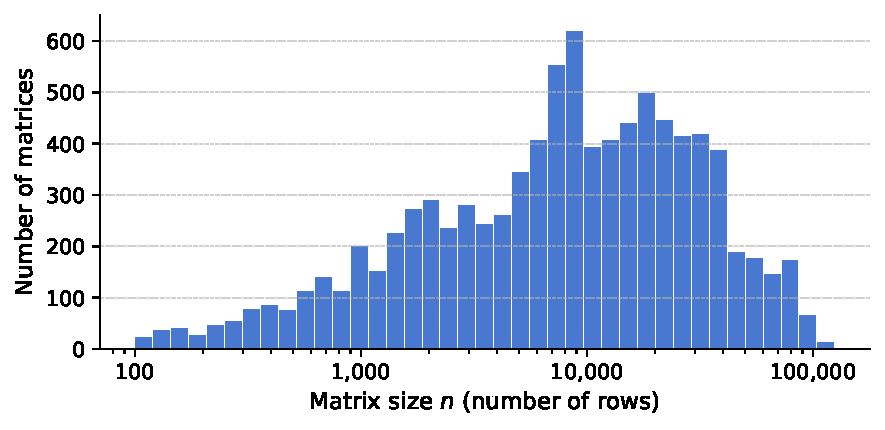
\includegraphics[width=0.85\textwidth]{figures/dataset_size_histogram.pdf}
  \caption{Distribution of matrix sizes (number of rows $n$) for the main thesis dataset
           (9{,}711 matrices, Campaigns~1--4). The $x$-axis uses a logarithmic scale.}
  \label{fig:dataset-sizes}
\end{figure}

\section{Feature Engineering}\label{sec:features}

The matrix features provided to the MLP branch complement the visual information captured by the CNN, and the choice of features can independently influence prediction quality.
The next section introduces the feature sets used in this thesis and how they differ from the MM-AutoSolver approach.

\subsection{MM-AutoSolver Reference Features}\label{subsec:features-mm}

The MM-AutoSolver paper~\cite{xiong2025mmautosolver} extracts 17 numerical features from each
matrix, listed in Table~\ref{tab:features-mm}.
These features are used in the re-implemented baseline (\texttt{mm\_baseline}) to allow a direct
comparison under the paper's original feature assumptions.

\begin{table}[H]
  \centering
  \caption{17 numerical features used in MM-AutoSolver~\cite{xiong2025mmautosolver}.}
  \label{tab:features-mm}
  \begin{tabular}{clp{7cm}}
    \toprule
    \# & Name & Description \\
    \midrule
    0  & \texttt{row\_num}                  & Number of rows $n$ \\
    1  & \texttt{nnz}                       & Total number of non-zeros \\
    2  & \texttt{nnz\_ratio}                & Fill ratio $\mathit{nnz}/n^2$ \\
    3  & \texttt{nnz\_lower}                & Non-zeros in strict lower triangle \\
    4  & \texttt{nnz\_upper}                & Non-zeros in strict upper triangle \\
    5  & \texttt{nnz\_diagonal}             & Number of non-zero diagonal entries \\
    6  & \texttt{ave\_nnz\_row}             & Average non-zeros per row ($\mathit{nnz}/n$) \\
    7  & \texttt{max\_nnz\_row}             & Maximum non-zeros in any single row \\
    8  & \texttt{arr\_nnz\_rows}            & Variance of per-row non-zero counts \\
    9  & \texttt{max\_value}                & Maximum absolute off-diagonal entry \\
    10 & \texttt{max\_value\_diagonal}      & Maximum absolute diagonal entry \\
    11 & \texttt{diagonal\_dominance\_ratio}& Fraction of rows where $|a_{ii}| > \sum_{j \neq i}|a_{ij}|$ \\
    12 & \texttt{is\_symmetry}              & 1 if $\|A - A^\top\|_F / \|A\|_F < 0.01$, else 0 \\
    13 & \texttt{pattern\_symmetry}         & Fraction of non-zero positions mirrored in $A^\top$ \\
    14 & \texttt{value\_symmetry}           & $1 - \|A - A^\top\|_F / \|A\|_F$ \\
    15 & \texttt{row\_variability}          & $\log(1 + \max_i(\max_j|a_{ij}| / \min_j|a_{ij}|))$ \\
    16 & \texttt{col\_variability}          & Same as above computed column-wise \\
    \bottomrule
  \end{tabular}
\end{table}

\subsection{Original 14 Features}\label{subsec:features-14}

The 14 features extracted from each matrix, shown in Table~\ref{tab:features-14}, are grouped by the matrix property they capture.
Features 0--2 describe size and sparsity (matrix dimension, non-zero count, and fill ratio).
Feature 3 captures symmetry via the asymmetry ratio.
Features 4 and 9 characterise diagonal dominance, which is relevant for the stability of ILU-based preconditioners~\cite{meijerink1977iterative, saad2003iterative}.
Features 5--8 encode magnitude and scaling information,
and features 10--13 capture structural properties such as bandwidth, diagonal fill, and row-norm variation.
While the covered property groups overlap with those in MM-AutoSolver,
the specific formulations differ in order to explore whether alternative encodings of the same matrix characteristics lead to better solver predictions.

\begin{table}[h]
  \centering
  \caption{Original 14 matrix features used in the single-channel experiments.}
  \label{tab:features-14}
  \begin{tabular}{cll}
    \toprule
    \textbf{\#} & \textbf{Name} & \textbf{Description} \\
    \midrule
    0  & $\log(1+n)$                     & Matrix size (number of rows) \\
    1  & $\log(1+\text{nnz})$            & Number of non-zero entries \\
    2  & $\text{nnz}/n^2$                & Density (fill ratio) \\
    3  & $\|A - A^\top\|_F / \|A\|_F$   & Asymmetry measure \\
    4  & $\text{mean}(|d_i| / \sum|r_i|)$ & Mean diagonal dominance \\
    5  & $\|A\|_F / n$                   & Frobenius norm per row \\
    6  & $\text{tr}(A) / n$              & Normalised trace \\
    7  & $\max|a_{ij}| / \text{mean}|a_{ij}|$ & Relative maximum entry \\
    8  & $\log(1 + \rho(A))$             & Log spectral radius \\
    9  & $\log(1 + \kappa_\text{diag})$  & Diagonal condition number proxy \\
    10 & $\text{bw} / n$                 & Normalised bandwidth \\
    11 & $\text{nnz}_\text{diag} / n$    & Fraction of non-zero diagonal entries \\
    12 & $\text{CV}(\|r_i\|)$            & Row norm coefficient of variation \\
    13 & $\|A - D\|_F / \|A\|_F$        & Off-diagonal Frobenius fraction \\
    \bottomrule
  \end{tabular}
\end{table}

\subsection{Extended 20-Feature Set}\label{subsec:features-20}

During experimentation, six additional features were introduced to address specific prediction weaknesses observed in Campaign~1,
expanding the feature vector to 20 entries (Table~\ref{tab:features-6}).
Features 14 and 15 improve the separation between CG-type and GMRES-type solvers by encoding the sign structure of off-diagonal
entries and the fraction of positive diagonal entries, both of which correlate with matrix definiteness~\cite{saad2003iterative}.
Feature 16 distinguishes structurally symmetric from truly asymmetric matrices, helping to separate \texttt{gmres+gamg} from \texttt{fgmres+gamg} predictions.
Features 17 and 19 target ILU preconditioner stability: the minimum per-row diagonal dominance detects the single worst-case
row for ILU breakdown, while the variance of dominance ratios captures patchy instability that the mean alone misses.
Feature 18 encodes whether the non-zero structure is grid-like or unstructured, which is a strong predictor of GAMG suitability~\cite{stuben2001review}.

\begin{table}[H]
  \centering
  \caption[Six additional matrix features introduced in Campaign~2.]{The 6 additional matrix features introduced in Campaign~2, expanding the feature vector from 14 to 20 entries.}
  \label{tab:features-6}
  \begin{tabular}{cll}
    \toprule
    \textbf{\#} & \textbf{Name} & \textbf{Description} \\
    \midrule
    14 & \texttt{neg\_offdiag\_frac}   & Fraction of off-diagonal entries that are negative \\
    15 & \texttt{pos\_diag\_frac}      & Fraction of strictly positive diagonal entries \\
    16 & \texttt{struct\_sym\_frac}    & Fraction of $(i,j)$ entries with a matching $(j,i)$ entry \\
    17 & \texttt{min\_diag\_dominance} & $\min_i |d_i| / \sum|a_{ij}|_{j \neq i}$ \\
    18 & \texttt{nnz\_per\_row\_cv}    & Coefficient of variation of per-row non-zero counts \\
    19 & \texttt{diag\_dom\_variance}  & Variance of per-row diagonal dominance ratios \\
    \bottomrule
  \end{tabular}
\end{table}

\section{Image Representations}\label{sec:image-modes}

Image representation is an interesting topic within the thesis approach of improving prediction accuracy,
as different downsampling methods store completely different data within the image later read by the CNN.
Thus, several different downsampling methods were implemented, as shown in Table~\ref{tab:image-modes}, including
the RCM (Reverse Cuthill--McKee) reordering~\cite{cuthill1969reducing} method which permutes matrix rows and columns to reduce bandwidth before rendering.
This reordering is applied solely for image generation and is not passed to the solver, as the original matrix is used unchanged during benchmarking.

\begin{table}[h]
  \centering
  \caption[The 14 image modes evaluated in the single-channel experiments.]{The 14 image modes evaluated in the single-channel experiments. The six \texttt{rcm\_*} variants apply Reverse Cuthill--McKee reordering to the matrix before rendering with the corresponding base mode.}
  \label{tab:image-modes}
  \begin{tabular}{lp{8.5cm}}
    \toprule
    \textbf{Mode} & \textbf{Description} \\
    \midrule
    \texttt{binary}           & 1 where any non-zero falls in a pixel cell, 0 elsewhere \\
    \texttt{density}          & Non-zero count per cell divided by cell area, normalised to $[0,1]$ \\
    \texttt{log\_density}     & $\log(1 + \text{count})$ per cell, normalised to $[0,1]$ \\
    \texttt{magnitude}        & Mean absolute entry value per cell, normalised to $[0,1]$ \\
    \texttt{sign}             & Mean sign per cell: positive $\to 1$, negative $\to 0$, mixed $\to 0.5$ \\
    \texttt{signed\_magnitude}& $\text{sign}(a) \cdot \log(1+|a|)$ per cell, normalised to $[0,1]$ with $0.5 = 0$ \\
    \texttt{symmetry}         & $|A - A^\top|$ per cell, normalised to $[0,1]$ \\
    \texttt{diagonal}         & Off-diagonal entries $= 0.5$, diagonal entries $= 1.0$ \\
    \midrule
    \texttt{rcm\_binary}           & \multirow{6}{*}{\parbox{8.5cm}{RCM-reordered variants of the above modes. Reverse Cuthill--McKee reordering reduces matrix bandwidth before rendering, grouping structurally related entries closer to the diagonal.}} \\
    \texttt{rcm\_density}          & \\
    \texttt{rcm\_log\_density}     & \\
    \texttt{rcm\_magnitude}        & \\
    \texttt{rcm\_sign}             & \\
    \texttt{rcm\_signed\_magnitude}& \\
    \bottomrule
  \end{tabular}
\end{table}

Throughout the thesis, experiments are referred to using the naming convention
\texttt{<mode>\_<size>} for single-channel and \texttt{<mode1>\_\_<mode2>\_<size>} for dual-channel experiments,
where \texttt{<size>} is the image resolution in pixels.
For example, \texttt{magnitude\_64} denotes magnitude downsampling at 64\,px,
and \texttt{magnitude\_\_rcm\_log\_density\_128} a dual-channel run with magnitude and
RCM log-density modes at 128\,px.

\section{Model Architecture}\label{sec:architecture}

The model consists of two sub-models combined into one prediction model.
The two branches are an MLP that processes previously defined matrix features, and a CNN that processes pre-rendered images.
Outputs are then concatenated and passed to a shared classification head, which produces the probability distribution over the 19 solver-preconditioner pairs.
Concatenation was chosen over element-wise addition as it is the more common fusion practice~\cite{baltruvsaitis2018multimodal} and gives the classification head greater freedom in weighting contributions from each branch independently.
Two different model sizes are introduced to evaluate the effect of model capacity.
The CNN branch supports a single image channel and a dual-channel variant that accepts two different images as input.

\subsection{CNN Branch}\label{subsec:cnn-branch}

The CNN branch accepts an image of the size $(C \times H \times W)$ as input,
where  $C = 1$ for single-channel and $C = 2$ for dual-channel experiments,
and $H = W \in \{64, 128\}$ depending on the image resolution.

The branch begins with an initial convolution block, a $3 \times 3$ convolution with
$c$ output channels, followed by batch normalisation~\cite{ioffe2015batch} and ReLU activation, and a
$2 \times 2$ max-pooling layer that halves the spatial dimensions.
This is then followed by two residual blocks (three for the large model variant),
where each one is separated by a $2 \times 2$ max-pooling step.
Each residual block consists of two $3 \times 3$ convolutions with batch normalisation
and a skip connection~\cite{he2016deep}: $\mathbf{y} = \text{ReLU}(\mathbf{x} + \text{block}(\mathbf{x}))$.

After the convolutional stack, an adaptive average pooling layer reduces the spatial
dimensions to a fixed $4 \times 4$ output regardless of input resolution.
The result is then flattened and passed through a fully connected layer to produce a
fixed-size CNN embedding of dimension $d_{\text{CNN}}$.

Two model sizes are defined:
\begin{itemize}
  \item \textbf{Small}: $c = 64$ channels, 2 residual blocks, $d_{\text{CNN}} = 256$,
        dropout $p = 0.3$, ${\approx}0.5$\,M parameters.
  \item \textbf{Large}: $c = 128$ channels, 3 residual blocks, $d_{\text{CNN}} = 512$,
        dropout $p = 0.4$, ${\approx}2$\,M parameters.
\end{itemize}

\subsection{MLP Branch}\label{subsec:mlp-branch}

The MLP branch processes the vector of scalar matrix features
$\mathbf{f} \in \mathbb{R}^{n_{\text{feat}}}$, where $n_{\text{feat}} \in \{14, 20\}$
depending on the experimental campaign.

It consists of two fully connected layers with ReLU activations:
\[
  \mathbf{h} = \text{ReLU}(W_2\,\text{ReLU}(W_1 \mathbf{f} + b_1) + b_2),
  \quad W_1, W_2 \in \mathbb{R}^{d_{\text{MLP}} \times \cdot}
\]
The hidden dimension is $d_{\text{MLP}} = 64$ (small model) or $d_{\text{MLP}} = 128$
(large model).
No dropout is applied in this branch, as the features are already low-dimensional and the risk of overfitting is low.

\subsection{Fusion and Classification Head}\label{subsec:fusion}

The outputs of the two branches are concatenated:
\[
  \mathbf{z} = [\mathbf{c}_{\text{CNN}};\, \mathbf{h}_{\text{MLP}}]
  \in \mathbb{R}^{d_{\text{CNN}} + d_{\text{MLP}}}
\]
and passed through a two-layer classification head with ReLU activation and dropout~\cite{srivastava2014dropout},
producing logits over the 19 solver-preconditioner classes:
\[
  \hat{\mathbf{y}} = W_{\text{out}}\,\text{ReLU}(W_{\text{head}}\,\mathbf{z} + b_{\text{head}}) + b_{\text{out}}
\]
The head hidden dimension is 128 (small) or 256 (large).

This concatenation-based fusion differs from the MM-AutoSolver~\cite{xiong2025mmautosolver} approach,
which uses an element-wise addition of the CNN and MLP outputs.
Concatenation is more flexible as the classification head here can learn arbitrary weighting
of the two branches, whereas element-wise addition requires both branches to produce
outputs with the same size and a compatible representation.

When \texttt{no\_cnn=True}, the CNN branch is disabled entirely and only the MLP branch
feeds into the head, serving as the \texttt{nocnn} feature-only baseline.

\section{Training Procedure}\label{sec:training}

All models are trained with the AdamW optimiser~\cite{loshchilov2019decoupled}
at a learning rate of $3 \times 10^{-4}$ and weight decay of $10^{-3}$.
A cosine annealing schedule~\cite{loshchilov2017sgdr} reduces the learning rate to zero over the full
training run of 256 epochs.
Batches of size 256, or in the dual-channel case 64 due to memory restrictions, are drawn
from the training split with shuffling.

The base loss is cross-entropy over the 19 classes.
In Campaigns~2 and~4 an additional convergence penalty is added:
\[
  \mathcal{L} = \mathcal{L}_{\text{CE}} + \lambda \sum_{k \notin \mathcal{C}(A)} \hat{p}_k
\]
where $\mathcal{C}(A)$ is the set of solvers that converged for matrix $A$,
$\hat{p}_k$ is the predicted probability for solver $k$, and $\lambda = 1.0$.
This directly penalises probability mass assigned to diverging solvers and is expected to reduce failure rates.

The dataset is split into 90\% training and 10\% validation data using a stratified split
with seed 42, ensuring each class is represented proportionally in both splits.
Checkpoints are saved every 5 epochs and the checkpoint from the final epoch is used for evaluation.
% !TeX root = ../main.tex
% Add the above to each chapter to make compiling the PDF easier in some editors.

\chapter{Experiments}\label{chapter:experiments}

This chapter presents the experiments conducted within the thesis and describes the key design choices
and the motivation behind each campaign.
Detailed results and metric comparisons are evaluated in \autoref{chapter:results}.

\section{Experimental Infrastructure}\label{sec:infra}

To ensure reproducibility, the whole pipeline runs within a Docker environment.
The pipeline includes distinct scripts for data generation, model training and model evaluation.
The training data is stored in HDF5 file format to enable fast access, and is shared across experiments unless stated otherwise.
Its generation was performed on an AMD Ryzen AI 7 350 and an AMD Ryzen 5 1600 Six-Core, described in more detail in \autoref{sec:dataset}
Checkpoints and logs are namespaced by experiment name and image size, allowing multiple runs to coexist without overwriting.
The training of the model for the different experiments was done on an NVIDIA GeForce RTX 5060 Laptop GPU.
All runs use a fixed random seed for reproducibility.
No special CPU configurations were done during data generation, since all solvers for a given matrix are benchmarked sequentially in the same process, core allocation variability affects their timings equally for a given matrix.
However, absolute timings and winner assignments remain hardware-dependent, and parallel solver configurations in particular may produce different results on machines with different core counts or memory layouts.

The full source code, configuration files, experiment logs and LaTeX sources that were used for the thesis are publicly available on GitHub\footnote{\url{https://github.com/Draggon01/IterativeSolverSelectionWithCNNs}} within the \texttt{Thesis-Submission} release marks the exact repository state at hand-in.

\section{Evaluation Metrics}\label{sec:metrics}

\subsection{Classification Metrics}\label{subsec:classification-metrics}

The experiment results are measured with four classification metrics, following the evaluation protocol of MM-AutoSolver~\cite{xiong2025mmautosolver}, to allow direct comparison:

\begin{itemize}
  \item \textbf{Accuracy (Acc)} - the fraction of test samples for which the predicted solver-preconditioner pair matches the best solver.
  \item \textbf{Macro Precision (MP)} - the average per-class precision across all 19 classes, weighted equally regardless of class size.
  \item \textbf{Macro Recall (MR)} - the average per-class recall, weighted equally across all classes.
  \item \textbf{Macro F1 (F1)} - the harmonic mean of macro precision and macro recall, balancing both measures into a single score.
\end{itemize}

Macro averaging is used rather than weighted averaging to treat all solver classes equally, which is important given the imbalanced class distribution in the dataset.

\subsection{Solver-Quality Metrics}\label{subsec:solver-quality-metrics}

If a predicted solver-preconditioner pair is not the best result but comes in as a close second, it will not be recognised
for the accuracy, which may not be ideal when targeting the implementation of the models within a specific pipeline.
For this case four additional metrics are introduced, which also give positive feedback if the chosen solver-preconditioner
pair is only marginally slower, just the second-best choice, or is extremely failure-resistant.

\begin{itemize}
    \item \textbf{Top-k accuracy (k=2,3)} - probability the predicted solver is within the top-k predictions. Top-3 accuracy is used as the primary quality metric in the results discussion, with near-optimal values available in the experiment summary files.
    \item \textbf{Near-optimal accuracy (k=5,10,20)} - the predicted solver is within k\% of the best solver time.
    \item \textbf{Mean Runtime Ratio (MRT×)} - the average ratio of the predicted solver's runtime to the best solver's runtime. A value of 1.0 means the predicted solver is always optimal; higher values indicate how much slower the predictions are on average. Samples where the predicted solver did not converge are excluded from the MRT calculation and counted in the failure rate instead, so the two metrics should be read together.
    \item \textbf{Failure rate} - the fraction of test samples where the predicted solver did not converge. This matters in practice because a non-converging solver must run to timeout before the failure is detected, which can be more costly than simply picking a slower but converging solver.
\end{itemize}

\subsection{Computational Cost}\label{subsec:compute-cost}

Training time and per-matrix inference cost (feature extraction and image rendering) are also recorded for each experiment.
Data generation time was not tracked.
These are reported in \autoref{chapter:results} alongside the classification metrics.

\subsection{Non-Learning Baselines}\label{subsec:baselines}

Two non-learning baselines are introduced as reference points.
\textbf{1-NN} and \textbf{5-NN} are $k$-nearest-neighbour classifiers that predict the best solver
by finding the most similar training matrices in the scalar feature space
(14-dimensional in Campaigns~1 and~3, 20-dimensional in Campaigns~2 and~4), without any CNN branch.
Additionally, a \textbf{nocnn} baseline disregards the CNN branch entirely,
learning only from the feature vector through the MLP and classification head.
This is used to isolate the contribution of the image input and allows the CNN's
value to be assessed independently of the feature branch.

\section{MM-AutoSolver Replication}\label{sec:mm-replication}

The first experiment replicates the results of the MM-AutoSolver~\cite{xiong2025mmautosolver} paper with a dataset that resembles the
dataset from the paper in solver-preconditioner distribution.
Due to the high computational cost of the benchmarking process for the 19 solver-preconditioner pairs that also scales significantly with matrix size,
the replication dataset is limited to matrices with up to 84{,}617 rows, compared to over one million rows in the original paper.
Table~\ref{tab:replication-distribution} compares the per-class sample counts of the replication dataset against the actual numbers of the paper.

Since the generator buckets were less targeted in the early stages, generation of certain classes took a significant amount of time.
Therefore, different classes are over- and underrepresented and the dataset remains skewed, but in different directions than the paper.

\begin{table}[H]
  \centering
  \caption{Per-class sample counts: MM-AutoSolver paper dataset vs.\ replication dataset used in this thesis.}
  \label{tab:replication-distribution}
  \begin{tabular}{lrrrr}
    \toprule
    \textbf{Solver} & \textbf{Ours} & \textbf{Ours\,\%} & \textbf{Paper} & \textbf{Paper\,\%} \\
    \midrule
    \texttt{fbcgsr+jacobi} & 2519 & 10.9 & 2173 & 18.7 \\
    \texttt{bcgsl+none}    & 2502 & 10.8 & 2054 & 17.7 \\
    \texttt{symmlq+icc}    &  162 &  0.7 & 1201 & 10.3 \\
    \texttt{symmlq+jacobi} &  211 &  0.9 &  923 &  7.9 \\
    \texttt{dgmres+none}   &   43 &  0.2 &  650 &  5.6 \\
    \texttt{gmres+gamg}    &  394 &  1.7 &  640 &  5.5 \\
    \texttt{cr+eisenstat}  & 2505 & 10.8 &  598 &  5.1 \\
    \texttt{symmlq+sor}    &  109 &  0.5 &  582 &  5.0 \\
    \texttt{fbcgsr+ilu}    & 1247 &  5.4 &  562 &  4.8 \\
    \texttt{minres+gamg}   &  412 &  1.8 &  524 &  4.5 \\
    \texttt{fcg+gamg}      &  143 &  0.6 &  342 &  2.9 \\
    \texttt{cr+jacobi}     & 2503 & 10.8 &  310 &  2.7 \\
    \texttt{cg+ilu}        & 2511 & 10.8 &  275 &  2.4 \\
    \texttt{fgmres+gamg}   &  146 &  0.6 &  226 &  1.9 \\
    \texttt{cg+eisenstat}  & 2525 & 10.9 &  224 &  1.9 \\
    \texttt{cg+bjacobi}    & 2503 & 10.8 &  193 &  1.7 \\
    \texttt{cr+ilu}        & 2500 & 10.8 &   68 &  0.6 \\
    \texttt{cgs+gamg}      &  106 &  0.5 &   49 &  0.4 \\
    \texttt{bcgsl+asm}     &  126 &  0.5 &   29 &  0.2 \\
    \midrule
    Total                  & 23{,}167 & 100.0 & 11{,}623 & 100.0 \\
    \bottomrule
  \end{tabular}
\end{table}

Figure~\ref{fig:replication-sizes} shows the distribution of matrix sizes in the replication dataset,
with sizes ranging from 100 to 84{,}617 rows and a median of 1{,}485.

\begin{figure}[H]
  \centering
  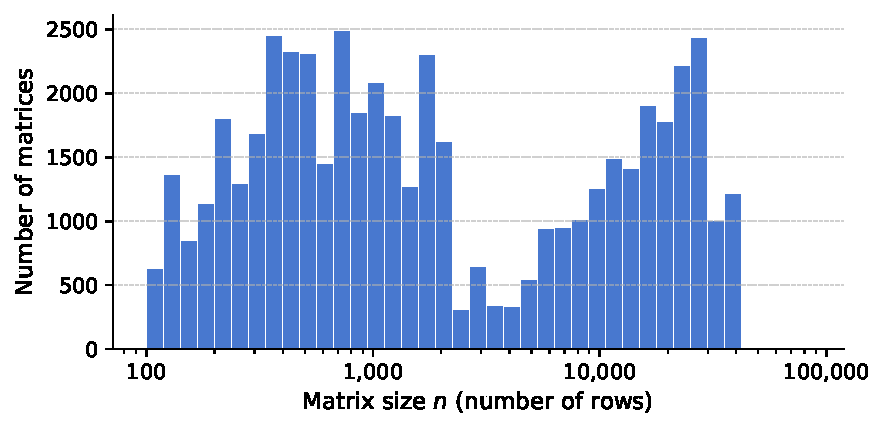
\includegraphics[width=0.85\textwidth]{figures/replication_size_histogram.pdf}
  \caption{Distribution of matrix sizes (number of rows $n$) for the MM-AutoSolver replication dataset
           (23{,}167 matrices). The $x$-axis uses a logarithmic scale.}
  \label{fig:replication-sizes}
\end{figure}

Following the paper, the experiment uses a $128 \times 128$ pixel density image for the CNN branch
and the 17 features proposed in the original work.
The re-implementation uses the original MM-AutoSolver architecture, two convolutional layers with Tanh activation
and element-wise CNN/MLP fusion, rather than the thesis model~(\autoref{sec:architecture}).
For the training, a learning rate of $10^{-3}$, $256$ training epochs and a batch size of $512$ are set.

\section{Single-Channel Experiments}\label{sec:single-channel-exp}

This section describes the different experiments done with a single CNN channel active.
They differ in their feature vector, the activation of the non-convergence penalty and model size.

\subsection{Campaign 1: Single-Channel Baseline}\label{subsec:campaign1}

The first experiment on the single branch is used to create a baseline for future experiment runs.
The 14 different image modes~(\autoref{sec:image-modes}) are tested to determine which of them carries the most useful information, and they are run on both 64\,px and 128\,px images.
Convergence penalty is deactivated and the small model~(\autoref{sec:architecture}) is used to establish a clean baseline.

\subsection{Campaign 2: Extended Features and Convergence Penalty}\label{subsec:campaign2}

Campaign 2 addresses two weaknesses observed in Campaign 1.
Some solvers had especially low accuracy and F1 values. An additional 6 features described in \autoref{tab:features-6} were therefore introduced.
To reduce high failure rates observed in certain classes, the convergence penalty~(\autoref{sec:training}) with $\lambda = 1.0$ is used.
The whole experiment is run on the large model~(\autoref{sec:architecture}) and uses the same image modes as Campaign 1 but only an image size of 64\,px.

\section{Dual-Channel Experiments}\label{sec:dual-channel-exp}

This section describes the experiments that use the dual-channel CNN approach.
To reduce computation time, only the best single-channel approach modes are combined with additional combinations included where
mode pairs are expected to capture complementary matrix information.

\subsection{Multimode HDF5 and Rendering Pipeline}\label{subsec:multimode-hdf5}

To evaluate dual-channel experiments efficiently, all required image modes are pre-rendered into a single shared HDF5 file
rather than maintaining separate per-experiment datasets.
The file stores one dataset per image mode under the key \texttt{images\_<mode>}, alongside the shared features, labels and runtimes from the original dataset.

\subsection{Campaign 3: Dual-Channel Approach}\label{subsec:campaign3}

The experiment setup is similar to the one in Campaign 1, except this time a different set of image modes and the large model~(\autoref{sec:architecture}) are used and
the image sizes are fixed at 64\,px.
Six image modes are selected from Campaign~1~(\autoref{subsec:campaign1}) based on F1 score and complementary information content, together with the sign mode.
These 7 methods are then combined into all their pairwise combinations and tested.
This results in 21 different image mode combinations that can be seen in Table~\ref{tab:results-campaign3}.

\subsection{Campaign 4: Dual-Channel with Extended Features}\label{subsec:campaign4}

This campaign combines the dual-channel approach with the improvements introduced in Campaign~2~(\autoref{subsec:campaign2}) with convergence penalty $\lambda = 1.0$, the 20-feature set and the large model~(\autoref{sec:architecture}).
The image modes are selected based on F1 performance in Campaign 2, and all selected mode pairs are run on both 64\,px and 128\,px.
This results in 15 different image mode combinations each run at two image sizes, giving 30 models in total.

\section{Ensemble Evaluation}\label{sec:ensemble}

\subsection{Campaign 5: Ensemble Method}\label{subsec:ensemble-method}

The ensemble combines independently trained models by averaging their predicted class probabilities before taking the final prediction.
No retraining is required as the member models are loaded from their saved checkpoints and are
evaluated on the shared validation split.

The shared multimode HDF5 (\autoref{subsec:multimode-hdf5}) ensures that all members
receive identical image data during ensemble inference.
Member selection follows two criteria: high individual F1 and complementary second
channels, so that the ensemble covers a wider range of matrix characteristics than
any single model.

For Campaign~3 the four ensemble members are (all 64\,px):
\begin{itemize}
  \item \texttt{magnitude+signed\_magnitude}
  \item \texttt{magnitude+rcm\_signed\_magnitude}
  \item \texttt{magnitude+symmetry}
  \item \texttt{rcm\_magnitude+signed\_magnitude}
\end{itemize}

For Campaign~4 the evaluated ensemble uses four members (all 128\,px):
\begin{itemize}
  \item \texttt{magnitude+log\_density}
  \item \texttt{magnitude+rcm\_log\_density}
  \item \texttt{rcm\_magnitude+rcm\_signed\_magnitude}
  \item \texttt{symmetry+log\_density}
\end{itemize}
These were selected for complementary first channels (magnitude $\times$2, \texttt{rcm\_magnitude}, symmetry)
and non-redundant second channels.


% !TeX root = ../main.tex
% Add the above to each chapter to make compiling the PDF easier in some editors.

\chapter{Results and Evaluation}\label{chapter:results}

This chapter presents and interprets the outcomes of the experiments described in \autoref{chapter:experiments}.
Each section addresses one research dimension: image mode choice, feature engineering, single- vs.\ dual-channel, image resolution, and ensembling,
before placing the best results in context with the MM-AutoSolver baseline.

\section{Overview of All Experimental Results}\label{sec:results-overview}

Each of the following sections presents its results table alongside the discussion, introducing metrics as they become relevant.
Bold marks the best value in each column; for Fail\% and MRT$\times$, lower is better.

\section{Impact of Image Mode}\label{sec:results-image-mode}

% ── Campaign 1: Single-channel, 14 features, no penalty ──────────────────────
\begin{table}[H]
  \centering
  \caption{Campaign~1 — Single-channel: 14 features, no convergence penalty, small model.}
  \label{tab:results-campaign1}
  \resizebox{\textwidth}{!}{%
  \begin{tabular}{lrrrrrrrr}
    \toprule
    \textbf{Experiment} & \textbf{Acc\%} & \textbf{MP\%} & \textbf{MR\%} & \textbf{F1\%} & \textbf{Top-2\%} & \textbf{Top-3\%} & \textbf{Fail\%} & \textbf{MRT$\times$} \\
    \midrule
    1-NN                     & 60.06 & 58.94 & 58.56 & 57.97 & 82.04 & 90.30 & 2.27 & 1.533 \\
    5-NN                     & 62.95 & 62.46 & 61.85 & 61.12 & 82.56 & 90.40 & 3.20 & 1.605 \\
    nocnn                    & 58.31 & 60.66 & 61.14 & 57.57 & 78.95 & 86.38 & 5.88 & 1.345 \\
    \midrule
    binary\_64               & 59.55 & 63.33 & 62.69 & 58.80 & 82.04 & 90.61 & 6.30 & 1.274 \\
    binary\_128              & 60.06 & 63.65 & 62.95 & 59.26 & 83.28 & 91.95 & 5.47 & 2.819 \\
    density\_64              & 60.27 & 63.17 & 62.29 & 59.46 & 81.42 & 91.54 & 5.47 & 1.291 \\
    density\_128             & 63.26 & 65.25 & 65.57 & 62.25 & 84.42 & 93.19 & 4.44 & 1.271 \\
    diagonal\_64             & 59.75 & 62.92 & 62.82 & 58.79 & 82.35 & 90.92 & 5.37 & 4.196 \\
    diagonal\_128            & 59.44 & 63.07 & 62.53 & 58.79 & 81.63 & 90.51 & 5.99 & 1.316 \\
    log\_density\_64         & 62.33 & 65.39 & 64.86 & 61.38 & 82.97 & 92.88 & 5.16 & 2.807 \\
    log\_density\_128        & 62.64 & 64.33 & 64.98 & 61.69 & 83.90 & 92.67 & 5.16 & 1.271 \\
    \textbf{magnitude\_64}   & \textbf{64.19} & 66.19 & \textbf{66.55} & \textbf{63.42} & \textbf{86.58} & 93.91 & 3.92 & 1.259 \\
    magnitude\_128           & 63.88 & \textbf{67.58} & 66.35 & 62.99 & 86.48 & 93.81 & 3.92 & 1.115 \\
    sign\_64                 & 60.37 & 63.08 & 62.59 & 59.29 & 82.25 & 91.64 & 5.68 & 1.288 \\
    sign\_128                & 61.20 & 65.11 & 64.28 & 60.53 & 83.08 & 92.16 & 4.02 & 4.139 \\
    signed\_magnitude\_64    & 62.85 & 64.56 & 65.20 & 61.68 & 84.83 & 94.22 & 4.75 & \textbf{1.069} \\
    signed\_magnitude\_128   & 61.82 & 64.75 & 64.53 & 60.42 & 84.73 & 93.09 & 5.06 & 1.222 \\
    symmetry\_64             & 62.95 & 64.40 & 65.66 & 61.85 & 85.66 & 94.01 & \textbf{3.51} & 4.081 \\
    symmetry\_128            & 62.95 & 64.14 & 65.32 & 61.62 & 85.96 & \textbf{94.43} & 4.64 & 1.233 \\
    \midrule
    rcm\_binary\_64          & 60.06 & 62.61 & 62.84 & 59.17 & 82.46 & 91.64 & 6.40 & 1.322 \\
    rcm\_binary\_128         & 59.86 & 62.18 & 62.40 & 59.01 & 82.35 & 91.64 & 6.81 & 1.269 \\
    rcm\_density\_64         & 61.40 & 64.53 & 64.09 & 60.43 & 83.59 & 93.40 & 5.68 & 1.235 \\
    rcm\_density\_128        & 62.33 & 65.47 & 64.84 & 61.33 & 82.77 & 93.29 & 4.75 & 1.262 \\
    rcm\_log\_density\_64    & 62.85 & 65.78 & 65.32 & 61.88 & 83.90 & 93.29 & 4.75 & 2.770 \\
    rcm\_log\_density\_128   & 61.82 & 63.55 & 64.19 & 60.94 & 83.49 & 92.36 & 5.47 & 1.271 \\
    rcm\_magnitude\_64       & 62.85 & 65.97 & 65.50 & 62.14 & 84.83 & 93.19 & 4.64 & 1.288 \\
    rcm\_magnitude\_128      & 63.05 & 65.93 & 65.35 & 62.55 & 84.62 & 92.67 & 4.13 & 1.281 \\
    rcm\_sign\_64            & 61.71 & 65.19 & 64.23 & 60.84 & 82.56 & 92.47 & 4.64 & 2.802 \\
    rcm\_sign\_128           & 61.82 & 65.53 & 64.63 & 61.05 & 82.77 & 92.98 & 4.23 & 2.829 \\
    rcm\_signed\_magnitude\_64  & 63.67 & 66.12 & 65.51 & 62.24 & 85.66 & 94.01 & 4.02 & 2.586 \\
    rcm\_signed\_magnitude\_128 & 63.36 & 64.74 & 65.65 & 62.23 & 85.35 & 94.12 & 4.64 & 1.235 \\
    \bottomrule
  \end{tabular}%
  }
\end{table}

% ── Campaign 2: Single-channel, 20 features, convergence penalty λ=1.0 ────────
\begin{table}[H]
  \centering
  \caption{Campaign~2 — Single-channel: 20 features, convergence penalty $\lambda=1.0$, large model, 64\,px.}
  \label{tab:results-campaign2}
  \resizebox{\textwidth}{!}{%
  \begin{tabular}{lrrrrrrrr}
    \toprule
    \textbf{Experiment} & \textbf{Acc\%} & \textbf{MP\%} & \textbf{MR\%} & \textbf{F1\%} & \textbf{Top-2\%} & \textbf{Top-3\%} & \textbf{Fail\%} & \textbf{MRT$\times$} \\
    \midrule
    1-NN                        & 59.44 & 59.02 & 58.34 & 57.00 & 82.15 & 90.40 & 1.86 & 1.539 \\
    5-NN                        & 63.57 & 63.25 & 62.38 & 61.61 & 82.97 & 91.02 & 2.89 & 1.589 \\
    nocnn                       & 59.75 & 62.40 & 62.72 & 59.08 & 80.80 & 89.78 & 4.95 & 2.926 \\
    \midrule
    binary\_64                  & 59.34 & 62.66 & 62.53 & 58.87 & 81.53 & 91.33 & 5.06 & 1.343 \\
    density\_64                 & 52.63 & 55.76 & 54.56 & 50.74 & 72.14 & 79.26 & 5.16 & 1.363 \\
    diagonal\_64                & 59.13 & 62.96 & 62.11 & 58.46 & 81.63 & 90.61 & 5.16 & 1.371 \\
    log\_density\_64            & 62.23 & 66.12 & 65.13 & 61.65 & 82.15 & 92.36 & 4.54 & 1.284 \\
    \textbf{magnitude\_64}      & \textbf{64.29} & 66.58 & \textbf{66.36} & \textbf{63.38} & \textbf{85.76} & 93.60 & 4.23 & 1.218 \\
    sign\_64                    & 60.99 & 64.54 & 63.49 & 60.19 & 83.08 & 93.60 & 4.44 & 1.304 \\
    signed\_magnitude\_64       & 61.20 & 63.39 & 62.78 & 59.85 & 85.24 & \textbf{94.01} & 5.16 & \textbf{1.068} \\
    symmetry\_64                & 63.36 & 64.74 & 65.49 & 61.94 & 85.04 & 93.81 & 3.72 & 1.254 \\
    \midrule
    rcm\_binary\_64             & 59.03 & 62.82 & 62.04 & 58.30 & 81.01 & 90.71 & 5.99 & 1.304 \\
    rcm\_density\_64            & 61.51 & 65.59 & 64.19 & 61.00 & 84.31 & 93.91 & 4.23 & 1.289 \\
    rcm\_log\_density\_64       & 62.75 & 66.52 & 65.27 & 62.12 & 82.56 & 92.26 & 4.75 & 1.264 \\
    rcm\_magnitude\_64          & 63.47 & \textbf{66.80} & 65.74 & 62.79 & 85.35 & 93.81 & \textbf{3.41} & 2.766 \\
    rcm\_sign\_64               & 61.51 & 65.43 & 63.82 & 60.87 & 81.94 & 91.95 & 4.23 & 1.326 \\
    rcm\_signed\_magnitude\_64  & 62.54 & 65.17 & 64.09 & 61.36 & 83.90 & 92.67 & 4.44 & 1.069 \\
    \bottomrule
  \end{tabular}%
  }
\end{table}

Across the first two Campaigns where single image modes were used, the magnitude\_64 downsampling is the strongest single predictor.
It consistently outperforms its 13 competitors, winning Campaign~1 (Table~\ref{tab:results-campaign1}) with a 64.19\% accuracy and a 63.42\% F1 value and
Campaign~2 (Table~\ref{tab:results-campaign2}) with a 64.29\% accuracy and a 63.38\% F1 value.

While in both Campaigns the magnitude\_64 downsampling approach yields better results than their best baseline approaches, there are always some
configurations where nearly no improvement or even worse values can be observed.
In Campaign~1, the binary\_64 model, for example, has a lower accuracy and only an F1 value 0.03\% higher than the 1-NN baseline, showing that
the binary downsampling does not store that much valuable information when cropped to small images.
In Campaign~2, the binary\_64 model also does not show better results, but within this campaign the density\_64 approach was more notable as it was the only one
that dropped by over 8\%.
Investigation showed the model stopped predicting \texttt{minres+gamg} and \texttt{fcg+gamg} entirely, which resulted in a failure rate of 0\%.
The convergence penalty pushed the model away from those high-failure-rate classes.
By never predicting them it avoided failures, but at the cost of reducing their recall to 0\%.
This shows that a low failure rate alone is not a sufficient signal and must be read together with per-class recall, indicating that the convergence penalty as currently implemented is not sufficient. This will be investigated further in \autoref{sec:results-features}.

As only a limited number of downsampling methods made sense, to introduce additional variations, RCM reordering was applied to selected modes.
This had no significant impact in single-channel model results as values in most cases stayed within $\pm 0.6$\% of the original values.

The worst-performing modes consist of those that only regard structural features like binary and diagonal
and do not incorporate any magnitude information, confirming that entry values carry essential information for solver selection.
The six highest-ranking modes by F1 - \texttt{magnitude}, \texttt{rcm\_signed\_magnitude}, \texttt{rcm\_magnitude},
\texttt{signed\_magnitude}, \texttt{symmetry}, and \texttt{density} - are therefore carried forward as the basis
for the dual-channel experiments in Campaign~3~(\autoref{subsec:campaign3}).

The results also show that if a model with exceptional speed needs to be selected, in most cases it won't be the model with the
highest accuracy or the best F1 value.
In Campaign~1 for example, \texttt{magnitude\_64} achieves the best accuracy and F1, but \texttt{signed\_magnitude\_64} has a lower mean runtime ratio (1.069 vs.\ 1.259), making it the better choice when minimising runtime overhead is the priority.

\section{Impact of Feature Engineering and Convergence Penalty}\label{sec:results-features}

Table~\ref{tab:results-campaign2} (shown above in \autoref{sec:results-image-mode}) covers Campaign~2.
From Campaign~1 to Campaign~2, six additional matrix features and the convergence penalty~(\autoref{sec:training}) with $\lambda=1.0$ were introduced.
Because no isolated ablation was run for the 20-feature approach with $\lambda=0$ and the 14-feature approach with
$\lambda=1.0$, the effects of these changes need to be discussed simultaneously.
Note that from this point on, all experiments use the larger model~(\autoref{sec:architecture}).

\paragraph{Accuracy impact}
The accuracy gains from Campaign~1 to Campaign~2 are modest.
The nocnn MLP-only baseline approach improves by 1.44\% to 59.75\%, suggesting that the new features add useful
information.
Since the penalty primarily shapes which solver classes the model avoids rather than the feature representation itself, the
expanded feature set is the more likely driver of this particular gain.
For CNN-based models the improvement is negligible, the best approach being magnitude, only shifts 0.10\% to 64.29\% in accuracy.
This shows that information from the new features might already be present in some way within the CNN representations,
which would explain the diminishing results in the CNN model approaches vs.\ the nocnn approach.

\paragraph{Failure rate impact}
The metric where the convergence penalty is most clearly visible is the failure rate.
Combined failure rates across single-channel experiments dropped from 3.5\%--6.8\% in Campaign~1 (Table~\ref{tab:results-campaign1}) to
3.4\%--6.0\% in Campaign~2 (Table~\ref{tab:results-campaign2}).
This shows that the overall failure rate drops, sometimes significantly.
When looking at the per-class results for the magnitude downsampling with 14 features and without the penalty versus the
20 features and penalty approach, before the penalty, 4 classes had failure rates above 10\%, after, only 2 remain.
Unfortunately, for \texttt{symmlq+sor} the failure rate surged from 14.8\% to 28.2\%, which then drops
the overall failure rate back to previous levels.
A likely explanation is that the convergence penalty suppressed other high-failure classes, as discussed further below,
causing their probability mass to be redistributed towards solvers such as \texttt{symmlq+sor}.

This behaviour is reproduced in the other models as well, therefore the penalty approach needs to be examined as to
not only provide a shift in failure rates but realistic improvement.

\paragraph{Density side-effect}
The main negative side effect in this experiment is that the \texttt{density\_64} model collapsed in accuracy, dropping to 52.63\% from previously 60.27\%.
This loss of over 10\,\% is only observed in this model and might indicate a training instability, as the drop was not reproduced in later experiments,
but may also hint that the density encoding and the penalty gradient do not interact well.

\paragraph{Convergence penalty improvement}
As discussed in \autoref{sec:results-image-mode}, the convergence penalty can cause the model to stop predicting certain classes entirely,
reducing their recall to 0\% while also dropping their failure rate to 0\%.
This happens because the current penalty fires on every training sample and discourages the model from assigning any probability to solvers that
did not converge for that matrix.
For classes like \texttt{minres+gamg} that fail on many matrices, this accumulates through the training and the model stops predicting them entirely in the end.

Therefore, the convergence penalty needs improvement in future work.
Two promising directions that might help reduce the downsides of the current convergence penalty are the usage of
a threshold-gate, only penalising predictions when they exceed a certain probability, or incorporating the runtime ratio into
the penalty calculation.

\section{Single-Channel vs.\ Dual-Channel}\label{sec:results-single-vs-dual}

Adding a second CNN channel consistently improves over the single-channel approaches.
The best single-channel model, \texttt{magnitude\_64} (Table~\ref{tab:results-campaign2}: 64.29\% accuracy, 63.38\% F1), is outperformed by
\texttt{magnitude\_\_log\_density\_64} (Table~\ref{tab:results-campaign4}: 65.94\% accuracy, 65.02\% F1).
The best overall model is \texttt{magnitude\_\_rcm\_log\_density\_128} with 66.56\% accuracy, a 2.27\,\% improvement
over the best single-channel approach.

The size of the gain depends strongly on which two channels are chosen. When their information encodes different properties
they excel the most.
This can be seen by the combination of \texttt{magnitude} (absolute values) with \texttt{log\_density} (structural density) or \texttt{rcm\_log\_density} (density after bandwidth reduction).
Pairs with similar information like \texttt{rcm\_log\_density\_\_log\_density\_128} (two log-family channels) often drop even below some single-channel approaches
if their single-channel performance was already weak.

This confirms that a second channel is useful but only if the two downsampling methods contain non-redundant information.

Across all dual-channel experiments the most important channel is \texttt{magnitude}, as it consistently appears in the best
dual-channel pairs, reaffirming that magnitude encodes discriminative information essential for solver selection.


\subsection{Dual-Channel Results Overview}\label{subsec:dual-chan-results}

% ── Campaign 3: Dual-channel, 14 features, large model, 64px, no penalty ──────
\begin{table}[H]
  \centering
  \caption{Campaign~3 — Dual-channel: 14 features, no convergence penalty, large model, 64\,px.}
  \label{tab:results-campaign3}
  \resizebox{\textwidth}{!}{%
  \begin{tabular}{lrrrrrrrr}
    \toprule
    \textbf{Experiment} & \textbf{Acc\%} & \textbf{MP\%} & \textbf{MR\%} & \textbf{F1\%} & \textbf{Top-2\%} & \textbf{Top-3\%} & \textbf{Fail\%} & \textbf{MRT$\times$} \\
    \midrule
    1-NN                                           & 60.06 & 58.94 & 58.56 & 57.97 & 82.04 & 90.30 & 2.27 & 1.533 \\
    5-NN                                           & 62.95 & 62.46 & 61.85 & 61.12 & 82.56 & 90.40 & 3.20 & 1.605 \\
    nocnn                                          & 60.06 & 63.20 & 62.71 & 59.37 & 80.91 & 89.37 & 6.19 & 1.289 \\
    \midrule
    density\_\_rcm\_magnitude\_64                   & 64.40 & 67.28 & 65.93 & 63.72 & 85.66 & 93.40 & 5.06 & 1.219 \\
    density\_\_sign\_64                             & 63.98 & 66.90 & 66.42 & 63.14 & 85.35 & 94.12 & 4.44 & 1.217 \\
    density\_\_signed\_magnitude\_64               & 61.82 & 64.35 & 63.66 & 60.52 & 84.42 & 93.19 & 4.54 & 1.227 \\
    density\_\_symmetry\_64                        & 63.57 & 63.78 & 66.09 & 62.98 & 85.96 & 94.12 & 3.61 & 1.796 \\
    magnitude\_\_density\_64                        & 64.50 & 68.09 & 67.13 & 63.95 & \textbf{87.41} & 94.43 & 4.23 & 1.215 \\
    magnitude\_\_rcm\_magnitude\_64                 & 64.40 & 66.64 & 65.89 & 63.24 & 85.24 & 92.98 & 4.13 & 1.244 \\
    \textbf{magnitude\_\_rcm\_signed\_magnitude\_64}& \textbf{66.05} & \textbf{69.25} & 67.64 & 64.79 & 86.79 & 94.22 & 2.89 & 3.920 \\
    magnitude\_\_sign\_64                           & 64.50 & 66.79 & 66.93 & 63.52 & 85.96 & 93.91 & 4.23 & 1.215 \\
    \textbf{magnitude\_\_signed\_magnitude\_64}     & \textbf{66.05} & 68.21 & \textbf{68.23} & \textbf{65.32} & 86.48 & 94.12 & \textbf{2.79} & 4.476 \\
    magnitude\_\_symmetry\_64                       & 65.63 & 67.20 & 67.59 & 64.66 & 84.83 & 93.40 & 3.61 & 1.258 \\
    rcm\_magnitude\_\_sign\_64                      & 64.91 & 66.97 & 67.04 & 64.03 & 85.66 & 94.22 & 4.13 & 1.229 \\
    rcm\_magnitude\_\_signed\_magnitude\_64         & 65.63 & 68.90 & 67.61 & 64.86 & 85.45 & 94.22 & 3.82 & 1.235 \\
    rcm\_magnitude\_\_symmetry\_64                  & 64.29 & 66.85 & 66.74 & 63.34 & 85.55 & \textbf{94.53} & 3.61 & 3.298 \\
    rcm\_signed\_magnitude\_\_density\_64           & 63.36 & 65.94 & 65.10 & 61.89 & 84.83 & 92.67 & 4.54 & \textbf{1.063} \\
    rcm\_signed\_magnitude\_\_rcm\_magnitude\_64    & 63.88 & 66.95 & 65.97 & 63.22 & 85.66 & 93.81 & 4.02 & 1.221 \\
    rcm\_signed\_magnitude\_\_sign\_64              & 62.44 & 65.12 & 64.14 & 60.79 & 84.93 & 93.70 & 4.33 & 1.226 \\
    rcm\_signed\_magnitude\_\_signed\_magnitude\_64 & 62.33 & 64.34 & 63.62 & 60.55 & 84.11 & 93.50 & 4.64 & 1.065 \\
    rcm\_signed\_magnitude\_\_symmetry\_64          & 62.85 & 63.05 & 64.26 & 61.81 & 83.49 & 92.26 & 3.82 & 1.631 \\
    signed\_magnitude\_\_sign\_64                   & 62.33 & 64.70 & 63.94 & 61.29 & 84.00 & 93.60 & 4.64 & 1.235 \\
    symmetry\_\_sign\_64                            & 63.05 & 65.83 & 65.22 & 61.92 & 85.66 & 93.91 & 3.72 & 3.093 \\
    symmetry\_\_signed\_magnitude\_64               & 63.36 & 64.72 & 64.92 & 62.08 & 85.96 & \textbf{94.53} & 3.20 & 1.930 \\
    \bottomrule
  \end{tabular}%
  }
\end{table}

% ── Campaign 4: Dual-channel, 20 features, convergence penalty λ=1.0 ──────────
\begin{table}[H]
  \centering
  \caption{Campaign~4 — Dual-channel: 20 features, convergence penalty $\lambda=1.0$, large model, 64\,px and 128\,px.}
  \label{tab:results-campaign4}
  \resizebox{\textwidth}{!}{%
  \begin{tabular}{lrrrrrrrr}
    \toprule
    \textbf{Experiment} & \textbf{Acc\%} & \textbf{MP\%} & \textbf{MR\%} & \textbf{F1\%} & \textbf{Top-2\%} & \textbf{Top-3\%} & \textbf{Fail\%} & \textbf{MRT$\times$} \\
    \midrule
    1-NN                                              & 59.44 & 59.02 & 58.34 & 57.00 & 82.15 & 90.40 & 1.86 & 1.539 \\
    5-NN                                              & 63.57 & 63.25 & 62.38 & 61.61 & 82.97 & 91.02 & 2.89 & 1.589 \\
    nocnn                                             & 59.75 & 62.40 & 62.72 & 59.08 & 80.80 & 89.78 & 4.95 & 2.926 \\
    \midrule
    magnitude\_\_log\_density\_64                     & 65.94 & 68.42 & 67.73 & 65.02 & 86.79 & 94.63 & 4.02 & 1.214 \\
    magnitude\_\_log\_density\_128                    & 65.94 & 68.67 & 68.22 & \textbf{65.60} & 87.00 & 94.63 & 4.13 & 1.051 \\
    magnitude\_\_rcm\_log\_density\_64                & 65.43 & 67.72 & 67.75 & 64.74 & 86.27 & 94.63 & 4.02 & 1.220 \\
    \textbf{magnitude\_\_rcm\_log\_density\_128}      & \textbf{66.56} & 69.15 & \textbf{68.88} & 65.53 & 86.38 & 94.53 & 3.51 & 1.051 \\
    magnitude\_\_rcm\_magnitude\_64                   & 63.78 & 66.49 & 65.76 & 63.37 & 86.27 & 94.63 & 3.92 & 1.227 \\
    magnitude\_\_rcm\_magnitude\_128                  & 65.02 & 66.73 & 66.62 & 64.22 & 87.10 & 94.74 & 3.61 & 1.222 \\
    magnitude\_\_rcm\_signed\_magnitude\_64           & 65.53 & 67.52 & 67.36 & 64.30 & 85.96 & 93.40 & 3.72 & 1.234 \\
    magnitude\_\_rcm\_signed\_magnitude\_128          & 65.84 & \textbf{69.39} & 67.59 & 65.16 & 86.38 & 94.43 & 3.72 & 1.213 \\
    magnitude\_\_symmetry\_64                         & 64.71 & 66.34 & 66.35 & 63.49 & 85.45 & 94.01 & \textbf{2.68} & 3.821 \\
    magnitude\_\_symmetry\_128                        & 64.60 & 66.86 & 66.41 & 63.87 & 85.55 & 93.81 & 3.61 & 1.086 \\
    rcm\_log\_density\_\_log\_density\_64             & 62.02 & 66.30 & 65.07 & 61.44 & 82.66 & 92.47 & 4.23 & 1.276 \\
    rcm\_log\_density\_\_log\_density\_128            & 63.26 & 66.32 & 65.71 & 62.28 & 84.73 & 94.32 & 4.64 & 1.223 \\
    rcm\_magnitude\_\_log\_density\_64                & 64.09 & 67.24 & 66.56 & 63.77 & 85.66 & 93.29 & 3.92 & 1.247 \\
    rcm\_magnitude\_\_log\_density\_128               & 64.60 & 67.97 & 67.00 & 64.35 & 86.17 & 93.91 & 4.02 & 1.227 \\
    rcm\_magnitude\_\_rcm\_log\_density\_64           & 63.98 & 66.95 & 65.98 & 63.51 & 85.35 & 93.40 & 3.82 & 1.256 \\
    rcm\_magnitude\_\_rcm\_log\_density\_128          & 64.50 & 68.06 & 67.03 & 64.19 & 84.52 & 93.19 & 3.51 & 1.282 \\
    rcm\_magnitude\_\_rcm\_signed\_magnitude\_64      & 64.29 & 67.98 & 66.25 & 63.50 & 85.55 & 94.53 & 4.02 & 1.218 \\
    rcm\_magnitude\_\_rcm\_signed\_magnitude\_128     & 64.60 & 67.94 & 66.77 & 64.30 & 86.79 & 94.32 & 4.02 & \textbf{1.048} \\
    rcm\_magnitude\_\_symmetry\_64                    & 63.67 & 64.68 & 65.37 & 62.66 & 86.17 & 94.43 & 3.20 & 2.765 \\
    rcm\_magnitude\_\_symmetry\_128                   & 65.02 & 66.05 & 66.83 & 64.23 & \textbf{87.20} & 94.84 & 2.99 & 3.063 \\
    rcm\_signed\_magnitude\_\_log\_density\_64        & 63.47 & 66.25 & 65.69 & 62.40 & 85.66 & 93.60 & 4.23 & 1.057 \\
    rcm\_signed\_magnitude\_\_log\_density\_128       & 63.36 & 66.43 & 65.51 & 62.54 & 86.27 & 94.53 & 4.13 & 1.228 \\
    rcm\_signed\_magnitude\_\_rcm\_log\_density\_64   & 64.40 & 66.05 & 65.84 & 63.42 & 85.96 & 94.12 & 3.92 & 1.072 \\
    rcm\_signed\_magnitude\_\_rcm\_log\_density\_128  & 63.67 & 66.50 & 65.11 & 62.52 & 85.86 & 94.01 & 4.02 & 1.263 \\
    symmetry\_\_log\_density\_64                      & 64.50 & 66.70 & 66.88 & 63.57 & 87.10 & 95.15 & 3.10 & 2.540 \\
    symmetry\_\_log\_density\_128                     & 65.12 & 66.68 & 67.14 & 64.10 & 86.79 & 94.84 & 3.10 & 3.336 \\
    symmetry\_\_rcm\_log\_density\_64                 & 64.29 & 67.12 & 66.69 & 63.43 & 85.66 & 94.01 & 3.10 & 4.058 \\
    symmetry\_\_rcm\_log\_density\_128                & 64.71 & 66.92 & 66.98 & 63.84 & 86.58 & \textbf{95.36} & 2.99 & 2.126 \\
    symmetry\_\_rcm\_signed\_magnitude\_64            & 64.09 & 65.96 & 65.58 & 62.62 & 84.31 & 93.29 & 3.20 & 1.817 \\
    symmetry\_\_rcm\_signed\_magnitude\_128           & 64.09 & 65.31 & 66.05 & 62.89 & 86.69 & 95.15 & 3.10 & 2.710 \\
    \bottomrule
  \end{tabular}%
  }
\end{table}

The dual-channel experiments are summarised in Table~\ref{tab:results-campaign3} (Campaign~3, 14 features, 64\,px)
and Table~\ref{tab:results-campaign4} (Campaign~4, 20 features, 64\,px and 128\,px).
For Campaign~3 the six best image modes from Campaign~1 - \texttt{magnitude}, \texttt{rcm\_signed\_magnitude},
\texttt{rcm\_magnitude}, \texttt{signed\_magnitude}, \texttt{symmetry}, and \texttt{density} -
together with \texttt{sign} are combined into all 21 pairwise combinations.
For Campaign~4 only the six best image modes from Campaign~2 - \texttt{magnitude}, \texttt{rcm\_magnitude},
\texttt{rcm\_log\_density}, \texttt{symmetry}, \texttt{log\_density}, and \texttt{rcm\_signed\_magnitude} - are combined,
yielding 15 pairs each evaluated at two resolutions (64\,px and 128\,px).

The dominant finding over these two Campaigns is that \texttt{magnitude} is the most informative channel in the dual-channel setting as well.
Every top-performing pair across both campaigns includes it as one channel.
Replacing \texttt{magnitude} with any other mode as the primary channel reduces accuracy by 2--3\,\%.

The best second channel is \texttt{log\_density} (best F1) or \texttt{rcm\_log\_density}
(best accuracy), both outperforming \texttt{symmetry} and \texttt{rcm\_signed\_magnitude}.
The combination \texttt{rcm\_log\_density+log\_density} (two log-family channels) performs
worst in Campaign~4, confirming that redundant modes do not benefit the model.

128\,px consistently outperforms 64\,px by $+0.5$--$+1.3$\,\% across all mode pairs,
at a cost of roughly $4\times$ longer training time and $4\times$ higher inference latency.
The best Campaign~4 single model is \texttt{magnitude+rcm\_log\_density} at 128\,px
with 66.56\% accuracy and 65.53\% F1.

Dual-channel models outperform the best single-channel model by $+2.3$\,\% in accuracy
(66.56\% vs.\ 64.29\%), confirming that the two image channels carry complementary
discriminative information beyond what either channel provides alone.

\section{Effect of Image Resolution}\label{sec:results-resolution}

In the dual-channel experiment with 64 and 128\,px images, shown in \autoref{tab:results-campaign4}, the increase in resolution
brings a consistent improvement of 0.5--1.3\,\% in accuracy and F1 values across all 15 mode pairs.
The largest gain is seen in \texttt{magnitude+rcm\_log\_density}, where accuracy improves by 1.13\,\% and F1 by 0.79\,\%.
The smallest gain is on \texttt{magnitude+log\_density}, where accuracy stays the same and only F1 increases by 0.58\,\%.
Almost all pairs improve or remain stable at higher resolution.

The cost of the higher resolution is a $4\times$ increase in inference time, as the dual-channel 64\,px model runs at approximately 2.8\,ms/sample and the
128\,px model takes about 10.9\,ms/sample.
The training time per model is around 13\,min at 64\,px and around 48\,min at 128\,px, on a NVIDIA GeForce RTX 5060 Laptop GPU.

In the single-channel experiments (Table~\ref{tab:results-campaign1}), results were more mixed.
\texttt{binary\_128} and \texttt{density\_128} outperformed their 64\,px counterparts, but for the magnitude mode the 64\,px version outperformed the 128\,px version in accuracy and F1.
This suggests that 64\,px is already sufficient for magnitude-encoded images, where per-cell absolute values matter more than the
fine spatial arrangement of non-zeros.

\section{Ensemble vs.\ Single Best Model}\label{sec:results-ensemble}

% ── Ensembles: Campaign 3 and Campaign 4 ─────────────────────────────────────
\begin{table}[H]
  \centering
  \caption{Campaign~5 - Ensemble results: averaging of four independently trained dual-channel models.
           \emph{Campaign~3}: 14 features, 64\,px, no penalty. Members are
           \texttt{mag+signed\_mag}, \texttt{mag+rcm\_signed\_mag},
           \texttt{mag+symmetry}, \texttt{rcm\_mag+signed\_mag}.
           \emph{Campaign~4}: 20 features, 128\,px, $\lambda=1.0$. Members are
           \texttt{mag+log\_density}, \texttt{mag+rcm\_log\_density},
           \texttt{rcm\_mag+rcm\_signed\_mag}, \texttt{symmetry+log\_density}.
           Bold marks the column best.}
  \label{tab:results-campaign5}
  \resizebox{\textwidth}{!}{%
  \begin{tabular}{lrrrrrrrr}
    \toprule
    \textbf{Ensemble} & \textbf{Acc\%} & \textbf{MP\%} & \textbf{MR\%} & \textbf{F1\%} & \textbf{Top-2\%} & \textbf{Top-3\%} & \textbf{Fail\%} & \textbf{MRT$\times$} \\
    \midrule
    Campaign~3 ensemble (64\,px, 4 models) & \textbf{67.39} & 69.47 & \textbf{69.58} & 66.37 & \textbf{87.82} & \textbf{94.94} & \textbf{2.79} & 4.055 \\
    Campaign~4 ensemble (128\,px, 4 models) & 67.29 & \textbf{70.37} & 69.48 & \textbf{66.77} & 87.41 & \textbf{94.94} & 3.92 & \textbf{1.043} \\
    \bottomrule
  \end{tabular}%
  }
\end{table}

\paragraph[Campaign 3 ensemble.]{Campaign~3 ensemble.}

The Campaign~3 ensemble (all 64\,px):
\begin{itemize}
  \item \texttt{magnitude+signed\_magnitude}
  \item \texttt{magnitude+rcm\_signed\_magnitude}
  \item \texttt{magnitude+symmetry}
  \item \texttt{rcm\_magnitude+signed\_magnitude}
\end{itemize}
achieves 67.39\% accuracy and an F1 of 66.37\%, surpassing the best individual member
(\texttt{magnitude+signed\_magnitude\_64} at 66.05\% accuracy and 65.32\% F1)
by $+1.34$\,\% in accuracy and $+1.05$\,\% in F1.
The failure rate drops to 2.79\%, below all four member models individually,
confirming that non-converging predictions are not correlated across members.

\paragraph[Campaign 4 ensemble.]{Campaign~4 ensemble.}
The Campaign~4 ensemble (all 128\,px):
\begin{itemize}
  \item \texttt{magnitude+log\_density}
  \item \texttt{magnitude+rcm\_log\_density}
  \item \texttt{rcm\_magnitude+rcm\_signed\_magnitude}
  \item \texttt{symmetry+log\_density}
\end{itemize}
achieves 67.29\% accuracy and 66.77\% F1, compared to the best individual member
\texttt{magnitude+rcm\_log\_density\_128} (66.56\% accuracy and 65.53\% F1),
a gain of $+0.73$\,\% in accuracy and $+1.24$\,\% in F1.
The failure rate of 3.92\% and mean runtime ratio of 1.043$\times$ remain below or comparable to all individual members.

Notably, the Campaign~4 ensemble surpasses the Campaign~3 ensemble only in F1 (66.77\% vs.\ 66.37\%),
while trailing in accuracy (67.29\% vs.\ 67.39\%).
This comes at notably higher inference cost, running at approximately 46.5\,ms/sample —
roughly $4\times$ slower than the Campaign~3 ensemble ($\approx$12\,ms) — due to the 128\,px images.

\paragraph{Inference cost.}
The ensemble multiplies inference time by the number of members ($4\times$).
At $\approx$12\,ms/sample for four dual-channel 64\,px models (Campaign~3) and
$\approx$46.5\,ms/sample for four dual-channel 128\,px models (Campaign~4), the
prediction overhead remains negligible compared to typical iterative solver runtimes
which range from tens of milliseconds to several seconds per solve.

\section{Comparison to MM-AutoSolver}\label{sec:comparison-mm}

This section compares the thesis model against the MM-AutoSolver paper results and the replication performed as a baseline.
The replication was trained on a synthetic dataset with some real SuiteSparse matrices included, but was
evaluated on the same 19 solver classes with slightly different per-class distributions.
The replication even exceeds the paper in accuracy by 3.43\,\%, as seen in \autoref{tab:comparison-mm}, and
may be the result of the slightly different data source~(\autoref{sec:dataset}).
\begin{table}[H]
  \centering
  \caption{Comparison against MM-AutoSolver~\cite{xiong2025mmautosolver}.
           Best model: \texttt{magnitude+rcm\_log\_density} at 128\,px (Campaign~4).
           Ensemble C3: 4 models, 64\,px, 14 features.
           Ensemble C4: 4 models, 128\,px, 20 features, $\lambda=1.0$.
           Bold marks the best thesis result in each column.}
  \label{tab:comparison-mm}
  \begin{tabular}{lrrrr}
    \toprule
    \textbf{System} & \textbf{Acc\%} & \textbf{MP\%} & \textbf{MR\%} & \textbf{F1\%} \\
    \midrule
    MM-AutoSolver (paper)              & 78.54 & 63.41 & 62.81 & 62.53 \\
    MM-AutoSolver (replication)        & 81.97 & 62.88 & 61.83 & 60.45 \\
    \midrule
    This thesis (best model, C4)      & 66.56 & 69.15 & 68.88 & 65.53 \\
    This thesis (ensemble C3, 64\,px)  & \textbf{67.39} & 69.47 & \textbf{69.58} & 66.37 \\
    This thesis (ensemble C4, 128\,px) & 67.29 & \textbf{70.37} & 69.48 & \textbf{66.77} \\
    \bottomrule
  \end{tabular}
\end{table}

A direct comparison between the MM-AutoSolver approach and the thesis approach is misleading for two reasons.
First, the class distribution in the dataset differs substantially from the MM-AutoSolver dataset, where the \texttt{fbcgsr+jacobi} and \texttt{bcgsl+none} classes make up more than 36\% of the whole distribution.
A model can exploit this by defaulting to one of these dominant classes when uncertain, inflating accuracy.
The thesis dataset was constructed with a minimal per-class constraint of 250 matrices and capped at 600 matrices per class,
resulting in a much flatter distribution and harder problem.
Second, the training matrices also differ, as the MM-AutoSolver paper uses more real-world application matrices generated
within FreeFEM~\cite{hecht2012freefem} and OpenFOAM~\cite{weller1998tensorial}.
In this thesis, only SuiteSparse matrices with real-world applications are used, while the remainder consists of synthetically generated ones.

Despite the lower accuracy, the macro-averaged metrics are less sensitive to class distribution and can still be compared.
The thesis model even achieves around 7\,\% better results in Macro Precision and Macro Recall, meaning that despite the harder
problem it learned to distinguish the classes better than the MM-AutoSolver approach.

Another insight is the Top-3 accuracy of around 94\%, meaning that even when the predicted solver is not the best,
in nearly all cases it is among the top three choices.
Combined with an average failure rate of around 3--4\%, the approach is practically viable.

\section{Per-Solver Analysis}\label{sec:per-solver}

\autoref{tab:per-solver-ensemble} breaks down per-class F1, precision, recall, and failure rate
for the Campaign~4 ensemble (members: \texttt{magnitude+log\_density},
\texttt{magnitude+rcm\_log\_density}, \texttt{rcm\_magnitude+rcm\_signed\_magnitude},
\texttt{symmetry+log\_density}; 20 features, 128\,px, $\lambda=1.0$; 67.29\% Acc, 66.77\% F1).
The 19 classes span a wide performance range, from \texttt{minres+gamg} at 88.7\% F1 down to
\texttt{gmres+gamg} at 20.9\% F1, illustrating that solver prediction difficulty varies
considerably across the label space.


\begin{table}[H]
  \centering
  \caption[Per-class results for the Campaign~4 ensemble.]{Per-class results for the Campaign~4 ensemble (4 models: magnitude+log\_density,
           magnitude+rcm\_log\_density, rcm\_magnitude+rcm\_signed\_magnitude,
           symmetry+log\_density, 128\,px, $\lambda=1.0$).
           Sorted by F1 descending. N is the number of training samples per class.}
  \label{tab:per-solver-ensemble}
  \begin{tabular}{lrrrrr}
    \toprule
    \textbf{Solver pair} & \textbf{N} & \textbf{F1\%} & \textbf{Prec\%} & \textbf{Rec\%} & \textbf{Fail\%} \\
    \midrule
    minres+gamg      &  600 & 88.7 & 80.8 & 98.3 &  0.0 \\
    cr+eisenstat     &  600 & 88.3 & 96.1 & 81.7 &  0.0 \\
    symmlq+sor       &  250 & 86.3 & 84.6 & 88.0 & 15.4 \\
    symmlq+jacobi    &  253 & 82.1 & 74.2 & 92.0 &  3.2 \\
    bcgsl+asm        &  428 & 73.4 & 78.4 & 69.0 &  2.7 \\
    fbcgsr+jacobi    &  600 & 72.3 & 72.9 & 71.7 &  1.7 \\
    cr+ilu           &  600 & 72.1 & 71.0 & 73.3 &  6.5 \\
    cr+jacobi        &  600 & 71.9 & 75.9 & 68.3 &  0.0 \\
    cg+bjacobi       &  600 & 71.9 & 67.6 & 76.7 &  4.4 \\
    cg+eisenstat     &  600 & 70.7 & 73.2 & 68.3 &  0.0 \\
    bcgsl+none       &  600 & 70.0 & 70.0 & 70.0 &  0.0 \\
    dgmres+none      &  354 & 66.7 & 64.9 & 68.6 &  0.0 \\
    symmlq+icc       &  600 & 63.8 & 56.4 & 73.3 &  5.1 \\
    fbcgsr+ilu       &  600 & 63.4 & 78.0 & 53.3 &  0.0 \\
    cgs+gamg         &  336 & 52.8 & 38.4 & 84.8 &  0.0 \\
    fcg+gamg         &  290 & 52.3 & 39.0 & 79.3 &  3.4 \\
    cg+ilu           &  600 & 52.1 & 52.5 & 51.7 & 30.5 \\
    fgmres+gamg      &  600 & 49.0 & 63.2 & 40.0 &  0.0 \\
    gmres+gamg       &  600 & 20.9 &100.0 & 11.7 &  0.0 \\
    \bottomrule
  \end{tabular}
\end{table}

\paragraph{Easy classes.}
\texttt{minres+gamg} (88.7\% F1, recall 98.3\%) leads the ranking, reliably identifying
symmetric indefinite problems that are unsuitable for CG-type solvers.
\texttt{cr+eisenstat} (88.3\% F1, precision 96.1\%) follows closely, dominating structurally
symmetric and nearly diagonally dominant matrices.
\texttt{symmlq+jacobi} (82.1\% F1, recall 92.0\%) shows high recall but lower precision
(74.2\%), indicating the model confidently identifies this class but occasionally predicts
it for matrices belonging to neighbouring symmetric solver classes.

\paragraph{Hard classes.}
\texttt{gmres+gamg} is the hardest class (20.9\% F1) with a recall of only 11.7\%
despite perfect precision of 100.0\%: the model is always right when it predicts this class,
but almost never does so.
This is a consequence of class ambiguity within the GAMG-preconditioned family:
\texttt{fgmres+gamg} (49.0\% F1) and \texttt{fcg+gamg} (52.3\% F1) converge in similar
time on many of the same matrices, and the model spreads probability across the family
rather than committing to one member.
\texttt{fbcgsr+ilu} (63.4\% F1, recall 53.3\%) and \texttt{symmlq+icc} (63.8\% F1) are
the next weakest: both are specialised combinations whose winning conditions are narrow
and hard to separate from neighbouring classes by image alone.

\paragraph{Failure rates.}
\texttt{cg+ilu} stands out with a 30.5\% failure rate, while \texttt{symmlq+sor} (15.4\%) and \texttt{cr+ilu} (6.5\%) also carry elevated rates.
All three rely on preconditioners sensitive to matrix conditioning, making them harder to predict reliably.
Despite these per-class spikes, the overall ensemble failure rate remains low at 3.92\%.

\section{Practical Inference Cost}\label{sec:inference-cost}

Model inference is fast enough to be negligible compared to actual solver runtimes.
\autoref{tab:inference-latency} summarises the per-sample CPU latency for the main model configurations, measured on the
969 validation samples.

\begin{table}[h]
  \centering
  \caption{CPU inference latency per sample (averaged over 969 validation samples).}
  \label{tab:inference-latency}
  \begin{tabular}{lrr}
    \toprule
    \textbf{Configuration} & \textbf{Latency (ms/sample)} & \textbf{Model params} \\
    \midrule
    MLP only (nocnn)                              & $\approx$0.08 & $\approx$57\,K \\
    Single-channel CNN, small model (64\,px)      & $\approx$1.2  & $\approx$0.5\,M \\
    Single-channel CNN, small model (128\,px)     & $\approx$4.5  & $\approx$0.5\,M \\
    Single-channel CNN, large model (64\,px)      & $\approx$2.8  & $\approx$2.1\,M \\
    Dual-channel CNN, large model (64\,px)        & $\approx$3.0  & $\approx$2.1\,M \\
    Dual-channel CNN, large model (128\,px)       & $\approx$10.9 & $\approx$2.1\,M \\
    Campaign~3 ensemble (64\,px, 4 models)        & $\approx$12.0 & $4\times$2.1\,M \\
    Campaign~4 ensemble (128\,px, 4 models)       & $\approx$46.5 & $4\times$2.1\,M \\
    \bottomrule
  \end{tabular}
\end{table}

The MLP-only baseline runs at under 0.1\,ms per sample, confirming that the scalar feature branch alone imposes negligible overhead.
Adding the CNN increases latency to around 1--3\,ms for 64\,px models, while 128\,px models are roughly $4\times$ slower, consistent with the fourfold increase in pixel count.
The dual-channel configuration adds only marginal cost over the equivalent single-channel model (2.8\,ms vs.\ 3.0\,ms at 64\,px), meaning the second image channel comes at almost no additional inference expense.

\paragraph{Full pipeline cost.}
Model inference alone does not capture the full overhead: feature extraction and image rendering must also be accounted for.
To illustrate the combined cost, a small timing experiment is conducted on two representative matrix types, a 2D Poisson grid (SPD) and a random non-symmetric matrix, each at two sizes, $n \approx 50\text{k}$ and $n \approx 100\text{k}$.
This is not a systematic benchmark but a targeted measurement to show where the pipeline time is spent.
The non-symmetric matrices use 50 non-zeros per row, giving $\text{nnz} \approx 2.6\text{M}$ and $\text{nnz} \approx 5.1\text{M}$ respectively, compared to $\approx 250\text{k}$ and $\approx 500\text{k}$ for the Poisson grids.
All 19 solvers converge within 10\,s on the SPD matrices and 11 of 19 converge within 10\,s on each non-symmetric matrix, with the remaining 8 either failing to converge or running beyond the 10\,s kill threshold set for this experiment.
The random baseline simulates picking uniformly at random until a solver converges: each failed attempt costs its detection time (capped at 10\,s), and the expected number of failures before success scales with $n_\text{failed}/n_\text{success}$.

Table~\ref{tab:pipeline-breakdown} shows the complete breakdown for the best-performing models from Campaigns~3 and~4.

\begin{table}[H]
  \centering
  \caption{
    Full pipeline breakdown for \texttt{rcm\_signed\_magnitude\_\_density\_64} (C3, MRT$\times$\,=\,1.063)
    and \texttt{magnitude\_\_rcm\_log\_density\_128} (C4, MRT$\times$\,=\,1.051) across four test matrices.
    All times in ms; image rendering covers both channels.
    Solvers are killed after 10\,s; the random baseline uses a geometric retry model.%
  }
  \label{tab:pipeline-breakdown}
  \resizebox{\textwidth}{!}{
  \begin{tabular}{lrrrrrrrr}
    \toprule
    & \multicolumn{4}{c}{\textbf{C3: rcm\_signed\_magnitude\_\_density\_64 (14 feat, 64\,px)}}
    & \multicolumn{4}{c}{\textbf{C4: magnitude\_\_rcm\_log\_density\_128 (20 feat, 128\,px)}} \\
    \cmidrule(lr){2-5}\cmidrule(lr){6-9}
    & \textbf{SPD 50k} & \textbf{SPD 100k} & \textbf{NS 50k} & \textbf{NS 100k}
    & \textbf{SPD 50k} & \textbf{SPD 100k} & \textbf{NS 50k} & \textbf{NS 100k} \\
    \midrule
    Feature extraction (ms)      &   33 &   23 &    93 & 384    &   521 &   600 &  2{,}617 & 5{,}424 \\
    Image rendering, 2ch.\ (ms)  &   29 &   55 &   304 & 641    &    28 &    54 &    302 &   631 \\
    Model inference (ms)         &    3 &    3 &     3 &   3    &    11 &    11 &     11 &    11 \\
    \midrule
    \textbf{Pipeline overhead (ms)} & \textbf{65} & \textbf{81} & \textbf{400} & \textbf{1{,}028} & \textbf{560} & \textbf{665} & \textbf{2{,}930} & \textbf{6{,}066} \\
    Predicted solve, MRT$\times$ (ms) & 108 & 237 &  39 &  55   &  107 &  234 &     38 &    54 \\
    \textbf{Total (ms)}          & \textbf{173} & \textbf{318} & \textbf{439} & \textbf{1{,}083} & \textbf{667} & \textbf{899} & \textbf{2{,}968} & \textbf{6{,}120} \\
    \midrule
    Best solver (ms)             & 102 & 223 &  37 &  51   &  102 &  223 &     37 &    51 \\
    Random baseline (ms)         & 270 & 1{,}225 & 6{,}468 & 7{,}484 & 270 & 1{,}225 & 6{,}468 & 7{,}484 \\
    \textbf{Speedup vs.\ random} & \textbf{1.56$\times$} & \textbf{3.85$\times$} & \textbf{14.75$\times$} & \textbf{6.91$\times$}
                                 & \textbf{0.40$\times$} & \textbf{1.36$\times$} & \textbf{2.18$\times$} & \textbf{1.22$\times$} \\
    \bottomrule
  \end{tabular}%
  }
\end{table}

The dominant cost in the 20-feature set is feature~16, the structural symmetry fraction, which checks for matching $(i,j)$--$(j,i)$ non-zero pairs using set operations that scale with $\text{nnz}$.
It accounts for 506\,ms on the sparse SPD 50k matrix, 589\,ms on SPD 100k, and 2.5\,s and 5.2\,s on the two non-symmetric matrices, making it responsible for the vast majority of C4's extraction time in every case.
The 14-feature set avoids this computation entirely, giving C3 a decisive pipeline advantage.

C3 achieves a positive speedup over random selection in all four cases, ranging from 1.56$\times$ on the well-conditioned SPD 50k matrix to 14.75$\times$ on the non-symmetric 50k matrix where 8 of 19 solvers fail or are killed.
C4 is slower than random on the small SPD matrix (0.40$\times$), where the 561\,ms overhead alone exceeds the 270\,ms random baseline, but achieves a 1.36$\times$ speedup on the larger one, where solver runtimes are long enough to offset the 664\,ms overhead.
On non-symmetric matrices C4 recovers a modest speedup (2.18$\times$ and 1.22$\times$), but remains 5--7$\times$ slower than C3 in absolute terms.

Both models were selected for their low MRT$\times$ values (C3: 1.063, C4: 1.051), meaning the predicted solver is only marginally slower than optimal on average, so solver-selection quality is comparable between the two campaigns.
These results show that the 14-feature pipeline of Campaign~3 offers a better cost-quality trade-off across all tested matrix types and sizes as it consistently beats random selection and keeps the pipeline overhead below 1.1\,s even at $n = 100\text{k}$.
Campaign~4's 20-feature pipeline is only competitive when expected solver runtimes substantially exceed its extraction overhead, which itself scales with matrix density and size.

% !TeX root = ../main.tex
% Add the above to each chapter to make compiling the PDF easier in some editors.

\chapter{Conclusion}\label{chapter:conclusion}

\section{Summary of Findings}\label{sec:summary-findings}

This thesis investigated the use of convolutional networks for iterative solver selection on sparse linear systems.
The most important finding for the image representation is that the magnitude encoding consistently provides the best information
for the CNN branch, outperforming all other encoding strategies tested across all experiments.
The 14-feature set proved sufficient for the task,
as the six additional features yielded only marginal accuracy gains. This suggests that the CNN image already captures much of the information
the extra features encode.
The MM-AutoSolver architecture was successfully replicated on an independently constructed dataset, confirming the viability of the multimodal approach and
validating their results~(\autoref{sec:mm-replication}).
Extending the single CNN channel to a dual-channel approach, where complementary image encodings are processed in parallel, consistently improved both accuracy and F1 over the
single-channel approach.
An ensemble of four dual-channel models improved the results further, showing that independently trained models with different image mode combinations capture complementary information.
Furthermore, the convergence penalty was found to cause class avoidance rather than real failure rate reduction in some cases, with potential
improvements discussed in \autoref{sec:results-features}.
Overall, the thesis demonstrates that a multimodal approach can meaningfully improve solver selection over non-learning baselines,
given sufficient training data and compute.

\section{Contributions}\label{sec:final-contributions}

\begin{itemize}
  \item Replication of the MM-AutoSolver architecture on an independently
        constructed dataset, validating the multimodal approach.
  \item Design and evaluation of a custom residual CNN architecture in two
        model sizes, supporting both single- and dual-channel image input.
  \item Systematic comparison of 14 image downsampling strategies across both
        64\,px and 128\,px resolutions, identifying magnitude encoding as the
        most effective representation.
  \item Dual-channel CNN evaluation across 30 image mode combinations via a
        shared multimode HDF5 rendering pipeline, demonstrating consistent
        improvement over single-channel models.
  \item Ensemble evaluation of four dual-channel models, showing further
        accuracy and F1 gains through complementary model combination.
  \item Introduction and evaluation of 6 additional matrix features, showing
        that the original 14-feature set is largely sufficient.
  \item Analysis of the convergence penalty loss term, identifying a
        class-avoidance side-effect and suggesting directions for improvement.
  \item Evaluation of inference cost, confirming that prediction overhead
        remains negligible compared to typical iterative solver runtimes.
\end{itemize}

\section{Limitations}\label{sec:limitations}

The dataset, while sufficient for the experiments conducted, is limited in size and diversity.
The synthetic data distribution might not cover all real-world matrix types, and a larger variety of other sources for real-world matrices would be needed
to validate the findings more broadly.
Furthermore, only 19 fixed solver-preconditioner pairs from PETSc were evaluated, even though the full library has many more combinations to offer.
Hyperparameter search was limited to fixed learning rates and architecture depths, leaving potential performance improvements unexplored.
The accuracy drop observed in the \texttt{density\_64} model under the convergence penalty was not fully investigated, and only hypotheses on the cause were discussed.
Finally, the current approach uses hard labels based on the fastest converging solver; soft labels derived from runtime ratios could provide richer training signals.

\section{Future Work}\label{sec:future-work}

\begin{itemize}
  \item Investigation of the \texttt{density\_64} side-effect under the convergence penalty,
        for example through a lambda sweep or mode-specific penalty weights.
  \item An improved convergence penalty formulation, such as the squared penalty or a
        runtime-ratio-based penalty as proposed in \autoref{sec:results-features}.
  \item Soft-label training, where targets are derived from runtime ratios rather than
        a hard best-solver label, to provide richer training signal.
  \item A larger and more diverse dataset, incorporating additional SuiteSparse matrices
        and a wider variety of synthetic matrix types, to improve generalisation.
  \item Extension to larger image resolutions (e.g.\ 256\,px) or learned image encodings
        to capture finer structural detail.
  \item A generalisation study training on synthetic data and evaluating on pure
        SuiteSparse matrices to quantify the distribution shift.
  \item Online integration of the model as a lightweight inference module within the
        embedding-based evaluation pipeline~\cite{weng2026embedding}, to measure real-world solver selection benefit.
  \item Active learning strategies that query the solver oracle only for the most
        uncertain matrices, reducing data generation cost.
  \item Feature selection or pruning to identify a minimal subset of matrix statistics
        that retains high prediction accuracy at reduced extraction cost, informed by the
        per-feature timing analysis in \autoref{sec:inference-cost}.
\end{itemize}


\appendix{}

\microtypesetup{protrusion=false}

\listoffigures{}
\listoftables{}
\microtypesetup{protrusion=true}
\printbibliography{}

\end{document}
